\documentclass[12pt]{article}
\usepackage[utf8]{inputenc}
\usepackage[paper=letterpaper,margin=1.25in]{geometry}
\usepackage{graphicx} 
\graphicspath{ {figures/} } % all figures are in the 'figures' folder
\usepackage{float}
\usepackage{subcaption}
\usepackage{indentfirst}
\usepackage{setspace}
\usepackage{amsmath}
\usepackage{url}
\usepackage{array}

\newcolumntype{L}[1]{>{\raggedright\let\newline\\\arraybackslash\hspace{0pt}}m{#1}}
% Fix backwards double quotes
\usepackage [autostyle, english = american]{csquotes}
\MakeOuterQuote{"}
% set up clickable links in ToC
\usepackage{hyperref} % [hidelinks] to turn off hilights
\hypersetup{linktocpage, colorlinks=false, linktoc=all}

% add in dots for sections in ToC
\usepackage[titles]{tocloft}
\renewcommand\cftsecleader{\cftdotfill{\cftdotsep}}

% include subsections, etc.. in table of contents
\setcounter{tocdepth}{4}
\setcounter{secnumdepth}{4}
\usepackage[usenames,dvipsnames,svgnames,table]{xcolor}

%% CODE SNIPPET CONFIGURATION %%
\usepackage{listings}
% verilog code snippet configuration
\lstdefinestyle{Verilog}{
	language=Verilog,
	frame=single,
	breaklines=true,
	basicstyle=\ttfamily\footnotesize, %font and size
	numbers=left,
	numberstyle=\tiny\color{black},
	keywordstyle=\color{Blue}\ttfamily,
    commentstyle=\color{Green}\ttfamily,
    emph = [1]{`timescale},
    emphstyle = [1]{\color{Magenta}},
    emph = [2]{BUFG,ODDR2},
    emphstyle = [2]{\color{Maroon}},
	}  
% Matlab code snippet configuration
\definecolor{mygreen}{rgb}{0.11,0.67,0} % color values Red, Green, Blue
\definecolor{mylilas}{rgb}{0.67,0.22,0.95}
\lstdefinestyle{Matlab}{
   language=Matlab,
   frame=single,
   breaklines=true,
   keywords={break,case,catch,continue,else,elseif,end,for,function,
      global,if,otherwise,persistent,return,switch,try,while},
   basicstyle=\ttfamily\footnotesize, %font and size
   keywordstyle=\color{blue},
   commentstyle=\color{mygreen},
   stringstyle=\color{mylilas},
   emph = [1]{all},
   emphstyle = [1]{\color{mylilas}},
   numbers=left,
   numberstyle=\tiny\color{black},
   stepnumber=1,
   numbersep=10pt,
   backgroundcolor=\color{white},
   tabsize=4,
   showspaces=false,
   showstringspaces=false
}  
% C code 
\definecolor{Cpurp}{rgb}{0.5,0,0.38}
\definecolor{Cgreen}{rgb}{0.47,0.70,0.53}
\lstdefinestyle{C}{
   language=C,
   frame=single,
   breaklines=true,
   basicstyle=\ttfamily\footnotesize, %font and size
   keywordstyle=\color{Cpurp},
   emph = [1]{u8, u16, u32, XIOModule},
   emphstyle = [1]{\color{Cgreen}},
   commentstyle=\color{Green},
   stringstyle=\color{blue},
   numbers=left,
   numberstyle=\tiny\color{black},
   stepnumber=1,
   numbersep=10pt,
   backgroundcolor=\color{white},
   tabsize=4,
   showspaces=false,
   showstringspaces=false
}  
\lstset{%
  escapeinside={(*}{*)},%
}

\begin{document}

\pagenumbering{gobble} % turn off page numbering for the first few pages

\begin{titlepage}
	\centering
	%{\huge\bfseries Real-Time Remote Mapping\par}
	{\huge\bfseries FPGA-Based Real-Time SLAM\par}
	\vfill
	
\includegraphics[width=7cm]{WPI_Inst_Prim_FulClr.png} % also works with logo.pdf
	\vfill
	{\par\large A Major Qualifying Project Report Submitted to the Faculty of \par}
	\vspace{0.25cm}
	{\large Worcester Polytechnic Institute\par}
	\vfill
	{\large In partial fulfillment of the requirements for the \par}
	\vspace{0.25cm}
	{\large Degree of Bachelor of Science in Electrical \& Computer Engineering\par}
	\vfill
	{\large By: \par}
	\vspace{0.25cm}
	{\Large Georges Gauthier \\ John DeCusati \par} 
	\vfill
	{\large \today \par}
	\vfill
	{\begin{flushright} 
	\large Advisor: \\ \Large Professor R. James Duckworth
	\end{flushright}}
\end{titlepage} %%%% Title page %%%%
\newpage

\newgeometry{top=1in,bottom=1in,right=1in,left=1in} % change margins, set to double space
\doublespacing

\tableofcontents % create a table of contents
\newpage

\begin{small} % make the font smaller to accommodate for long figure names
\listoffigures % create a list of figures
\end{small}
\newpage 

\pagenumbering{roman} % change page numbering to i,ii, ...

%\phantomsection % makes clickable ToC link work
\addcontentsline{toc}{section}{Acknowledgements}
\section*{Acknowledgements}
text %%%% Acknowledgements %%%%
%\newpage

\phantomsection
\addcontentsline{toc}{section}{Abstract}
\section*{Abstract}
The overall goal of this project is to create a device capable of generating detailed maps and imagery of an area in real-time. This device will rely on an FPGA, and will use image processing algorithms capable of detecting, localizing, and tracking human beings. The device will gather imagery from the visual light and infrared-spectrums, as well as localization data and distance measurements from an IMU and a rangefinder. Along with gathering and processing data, the device will also serve as a long-range wireless access point, and will be able to transmit all generated maps and imagery in real-time. A major deliverable of this project is that the transmitted data will be fully processed, allowing it to be viewed remotely on less-powerful, mobile devices.
\par
This device will be especially useful for first responders. It is intended to be mounted on a small remote control vehicle, allowing any connected user to wirelessly traverse dangerous and remote locations in search of people in need. Since this device transmits data in real-time, it will be able to provide first responders with an accurate representation of not only a 2-D floor plan of an area such as a building, but also where any people are located. An anticipated use of this device would be in the event of a building in danger of collapsing. Since it would be dangerous to physically enter the building, first responders could locate any people trapped inside and find the fastest route to them using the wirelessly transmitted floorplan. The first responders would also be aware of any dangers in their way by making use of the real-time augmented video stream. This video stream will consist of image data with overlaid with object indicators and location information on any human beings detected by the image processing algorithms.
 
 %%%% Abstract %%%%
\newpage

\pagenumbering{arabic} % change page numbering to 1,2, ...

\section{Introduction}
In recent years, improvements in embedded processing technology have allowed for the creation of robotic situational awareness platforms for remotely observing dangerous or inaccessible areas. The market for such devices is a new and expanding field, and faces large demand from the military and first responders. This field is being piloted by throwable and remotely drivable platforms such as the Endeavor Robotics 110 FirstLook and the Bounce Imaging Explorer, shown in Figure \ref{robocop}. 

\par
\begin{figure}[H]
        \begin{subfigure}[h]{0.5\textwidth}
             \centerline{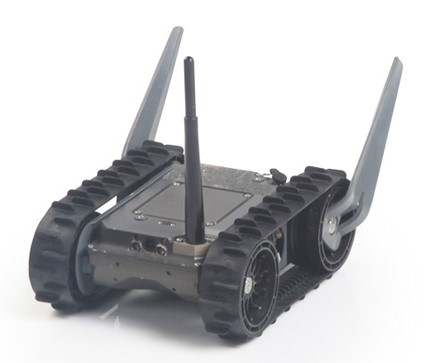
\includegraphics[width=1.0\textwidth]{FirstLook.jpg}}
            \caption{Endeavor Robotics 110 FirstLook \cite{endeavor}}
        \end{subfigure}
        \begin{subfigure}[h]{0.5\textwidth}
            \centerline{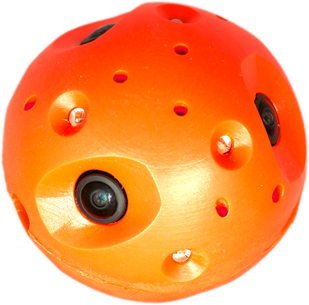
\includegraphics[width=0.8\textwidth]{bounce_img.png}}
            \caption{Bounce Imaging Explorer \cite{bounceImaging}}
        \end{subfigure}
\caption{Robotic Situational Awareness Devices}
\label{robocop}
\end{figure}
\par
These devices contain simple wireless video streaming technology, allowing for remote visual surveillance. Although a video stream is an effective strategy for simple surveillance, this method of gathering information has room for improvement. This project investigated the extraction of information such as object positioning and localization from a camera-based sensor suite in real time, allowing for more comprehensive situational observation. One method of performing this process is through the use of Simultaneous Localization and Mapping, or SLAM. 
\par
SLAM is a technique of mapping an unknown environment with respect to an agent, and can be performed using a wide variety of sensors and computational methods. This technique is a common area of research in the fields of image processing and high-speed computing, and has been applied mainly to autonomous vehicles. Most current SLAM implementations rely on the use of a sensor suite connected to a computer or System on Chip (SoC) computing device. 
\par
One type of technology useful for performing the high speed data processing necessary for an embedded SLAM device is a Field Programmable Gate Array, or FPGA. FPGAs consist of digital circuitry that is designed to be user-configured, allowing for the creation of completely customized digital hardware. FPGAs are especially useful for parallelized data processing, posing potential real-time advantages over standard computing or microcontroller technology. Although FPGA technology is highly applicable to performing SLAM-like tasks, there are currently few existing products that use FPGAs for this purpose. 
\par
This project explored the viability of an FPGA-based real-time SLAM sensor suite as a replacement for standard video cameras on existing situational awareness systems. This sensor suite utilized data from stereo camera modules, a scanning laser rangefinder, and an Inertial Measurement Unit (IMU) to create a real-time depth-augmented video feed and a 2D floorplan from the device's field of view.
\par
The following chapters detail the creation of this sensor suite, beginning with an exploration of relevant technology and prior work. Next, the overall system design of the project is included with a system block diagram. Then, each individual sensor’s implementation is explored in more detail. Methods for processing and combining sensor data to produce the intended 2D floorplan and 3D map visualizations are included. Comprehensive test results are then examined in detail for all sensors and main algorithms used. Lastly, conclusions and recommendations for future improvements are presented. 
 %%%% Introduction %%%%
\newpage

\section{Background}
The initial research portion of this project focused on learning more about different remote situational awareness products and how they may have been improved using existing technology, eventually leading to a set of overall project goals.

\subsection{Remote Situational Awareness Products}
Many situational awareness devices consist of remote-controlled throwable robots with wireless video-streaming capability. One such example is the 110 FirstLook by Endeavor Robotics, seen in Figure \ref{robocop}a. This device is a throwable, rugged robot that streams real-time video of its surroundings, and is used to investigate dangerous locations and hazardous material while keeping its operator out of harm's way. The 110 FirstLook has four day and night cameras, and also supports two-way audio. The device is remotely controlled by a tablet operator control unit, and is currently in use for military applications \cite{endeavor}.
\par
Similar to the 110 FirstLook, the Bounce Image Explorer is a throwable camera ball that wirelessly transmits a 360$^\circ$ real-time video stream of its surroundings. The Bounce Image Explorer can be seen in Figure \ref{robocop}b. The Explorer processes input from six monochrome WVGA camera modules, and outputs a video stream that can be accessed from a tablet or smartphone. This device is currently in a trial phase with United States Law Enforcement \cite{bounceImaging}. 
\par
A more commercial remote situational awareness device is the Serveball Squito\textsuperscript{TM} \cite{serveball}. Squito is a wireless, throwable, 360$^{\circ}$ panoramic camera that implements target detection to produce a stabilized output video stream. This device is shown in Figure \ref{squito} below.

\begin{figure}[H]
	\centerline{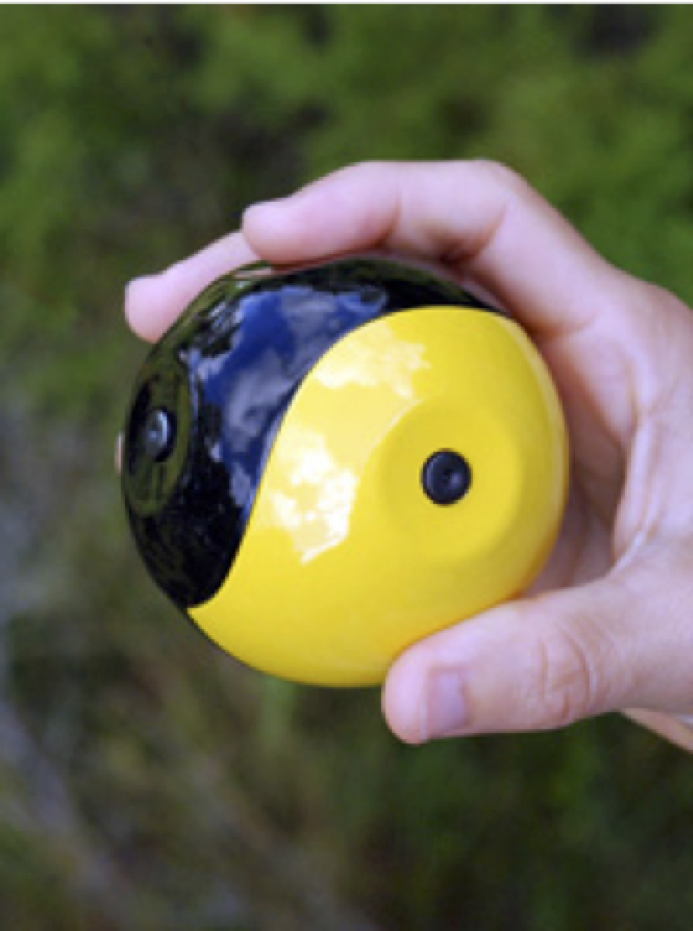
\includegraphics[width=0.3\textwidth]{serveball_squito.png}}
	\caption{Serveball's Squito \cite{serveball}}
	\label{squito}
\end{figure}

Squito utilizes a microprocessor receiving input from a fiber optic camera interface, as well as orientation and position sensors, in order to transmit a real-time stabilized video of its surroundings. The image in Figure \ref{squito_io} shows the input from the Squito's four camera inputs on the left, and a corresponding stitched output on the right. The device is still in the prototype stage, and has received interest from the first responder community. 
\par
\begin{figure}[H]
	\centerline{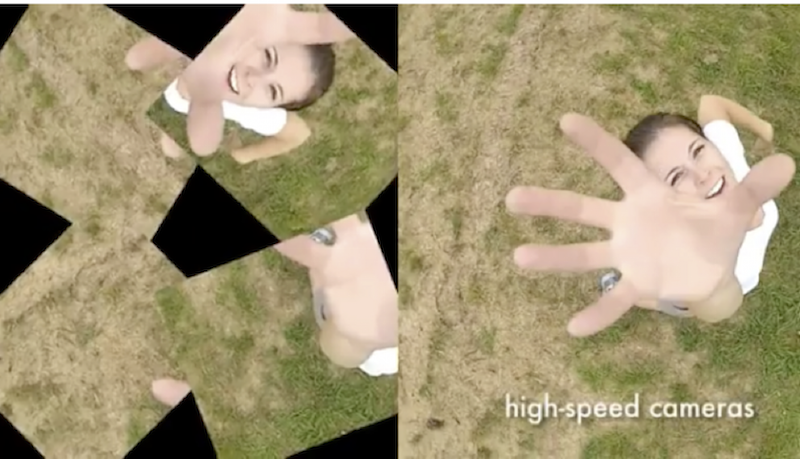
\includegraphics[width=0.6\textwidth]{serveball_io.png}}
	\caption{Serveball's Squito Input and Output \cite{serveball}}
	\label{squito_io}
\end{figure}
\par
The 110 FirstLook, Explorer, and Squito are all examples of remote situational awareness products that contain basic controls and real time video streaming outputs. Using additional image processing in the form of Simultaneous Localization and Mapping, the outputs of each of these devices could be improved to create comprehensive situational awareness. 

\subsection{Simultaneous Localization and Mapping}
As mentioned in the previous chapter, Simultaneous Localization and Mapping is the technique of mapping an unknown environment with respect to a localized agent. SLAM is especially useful for autonomous systems and remote observation, as it can be used for situational analysis and response. Recent research in the field of SLAM has focused on making these systems more portable.
\par
One application of such a system was a proof of concept of camera-based SLAM implementation for feature identification presented by Andrew Davison of Oxford University \cite{davison}. This system was handheld, and relied on a computer using a 2.2 GHz Pentium processor connected to a single camera and laser rangefinder. This system implemented edge detection on a known environment, and produced a real-time video output containing a 3D feature localization plot. An output frame from the device is shown in Figure \ref{rtSLAM}.

\begin{figure}[H]
	\centerline{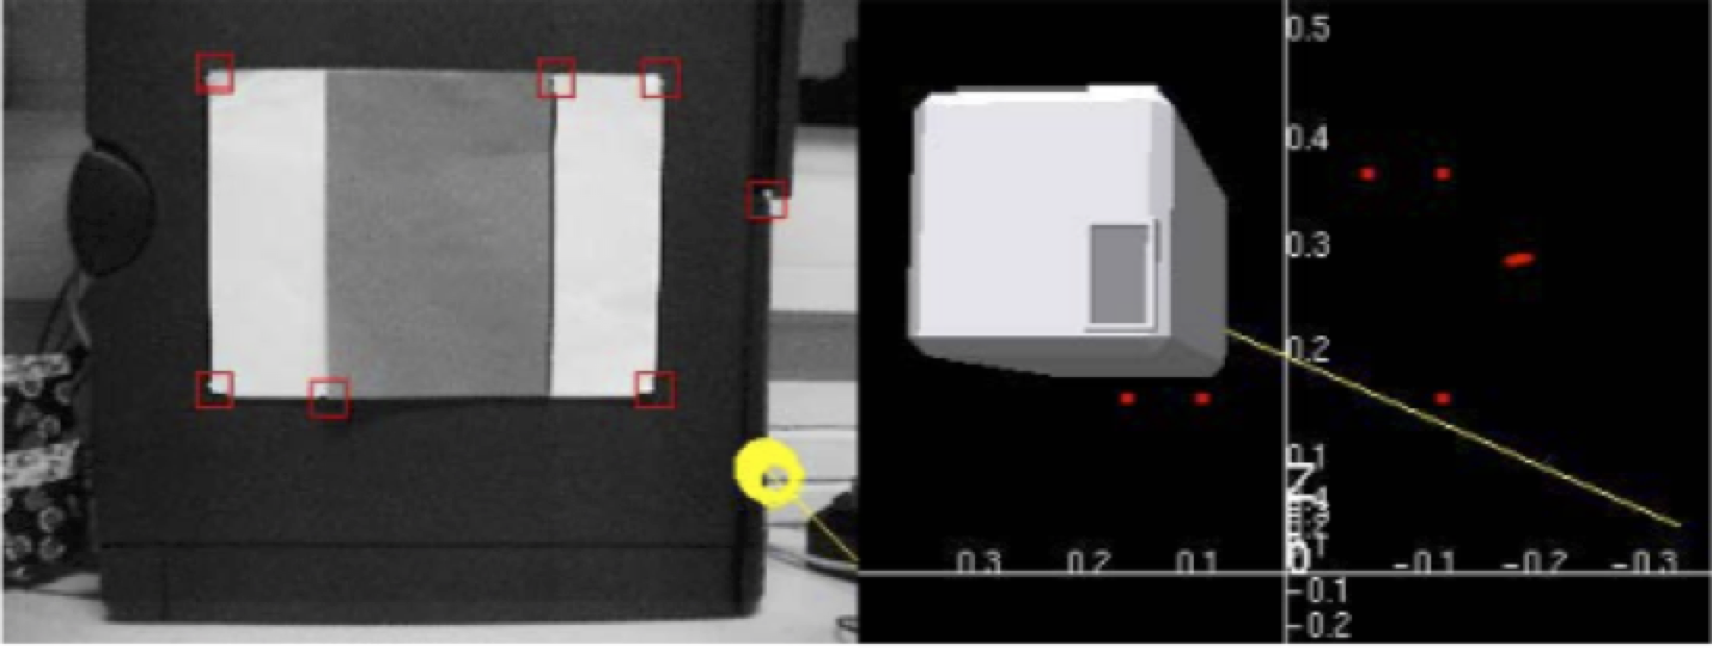
\includegraphics[width=0.8\textwidth]{real_time_SLAM.png}}
	\caption{Real-Time SLAM with a Single Camera \cite{davison}}
	\label{rtSLAM}
\end{figure}

The left image in Figure \ref{rtSLAM} shows 6 points of a paper target that were input to the system as prior knowledge, along with successfully marked identifying features (marked as red squares), and another identifying feature that was not marked for measurement (marked by a yellow circle). The frame on the right is a localization plot that displayed the relative positions of all red squares detected by the device.
\par
Along with identifying features of interest, SLAM image processing techniques are also used for depth estimation. The process of estimating depth from imagery is known as disparity mapping. Disparity mapping algorithms are used to calculate the similarities between stereo camera image pairs, and to convert said similarities to relative depth measurements. Disparity mapping is useful for situational awareness because it is used to determine the exact locations of all objects within a sensor suite's field of view.
\par
University of Bologna researchers Stefano Mattoccia and Matteo Poggi have worked to implement a real-time disparity mapping algorithm on an FPGA, and an example of a disparity image from this implementation is shown in Figure \ref{disparity_example} \cite{mattoccia}. Using their stereo disparity implementation, the researchers were able to generate real-time video showing the relative locations of objects within the device's field of view. The relative distance from the device to a given object was displayed using a color gradient, with nearer objects shown in brighter colors. Based on this depth information, it was also possible for the researchers to detect objects located within the field of view of the stereo imaging system, as shown in Figure \ref{disparity_example}. This implementation was extremely applicable to situational awareness systems, as it allowed for the localization of objects and creation of 2D slices of an area in real-time using only two camera sensors.
\par
\begin{figure}[H]
	\centerline{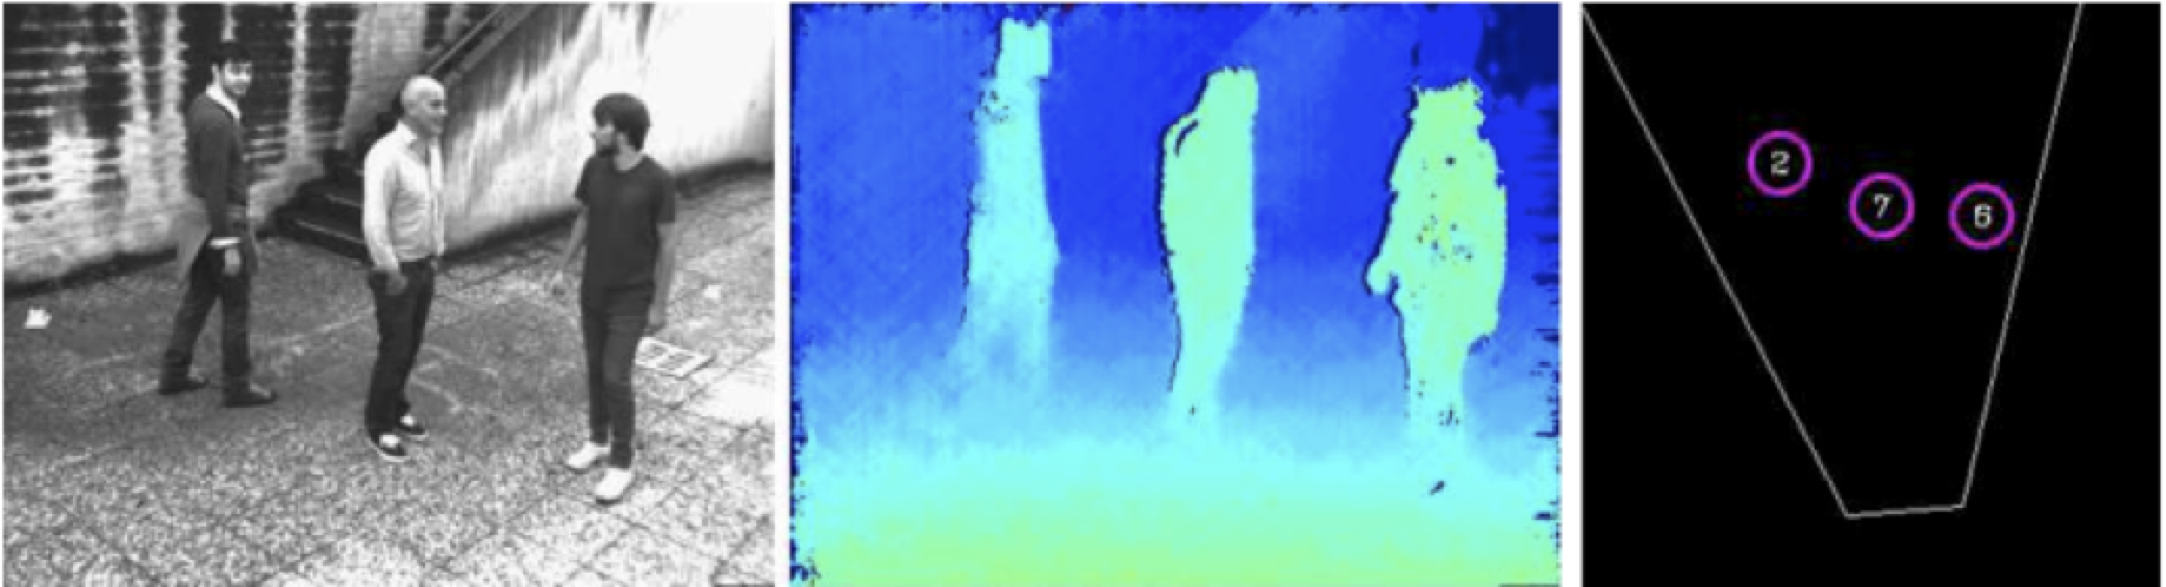
\includegraphics[width=0.9\textwidth]{disparity_example.png}}
	\caption{From Left to Right: Original Image, Disparity Map, Object Detection Results \cite{mattoccia}}
	\label{disparity_example}
\end{figure}
\par
A major concern with calculating disparity in real time is image processing speed. In the case of the implementation shown above, the parallelized data processing capabilities of FPGA hardware were used to address these concerns. The successful creation of this system demonstrated that FPGAs are useful for complex image processing applications \cite{mattoccia}. 

\subsection{The Zynq Evaluation and Development Board (ZedBoard)}
The FPGA platform used in this project was the Zynq Evaluation and Development Board, or ZedBoard. The ZedBoard is a low-cost development board containing a Xilinx Zynq-7000 All-Programmable SoC, and is shown in Figure \ref{zedboard_pic}.

\begin{figure}[H]
	\centerline{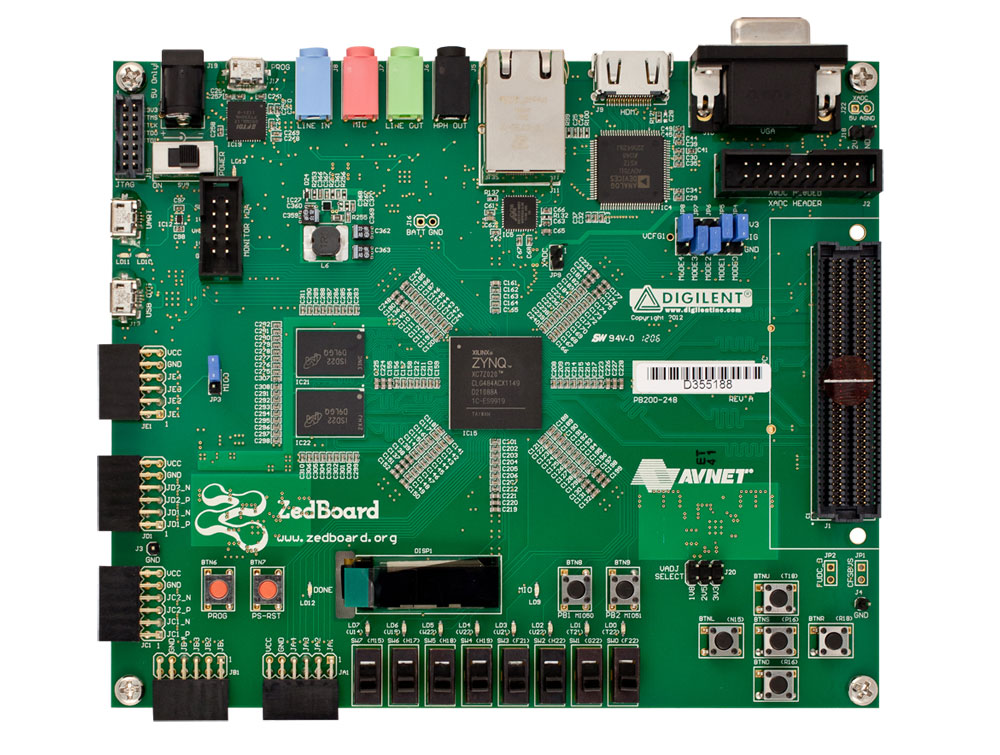
\includegraphics[width=1\textwidth]{ZedBoard.jpg}}
	\caption{The Avnet ZedBoard \cite{zedboard_photo}}
	\label{zedboard_pic}
\end{figure}

The Xilinx Zynq-7000 SoC consists of a dual-core ARM Cortex A9 processor coupled with Xilinx Artix-7 FPGA fabric. The ARM Cortex A9 processor uses a dedicated 33.3333 MHz clock source, while the onboard 100 MHz oscillator supplies the Programmable Logic (PL) clock. The Zynq-7000 SoC contains 85,000 programmable logic cells with 140 36K Block RAM modules. The ZedBoard also features 5 Pmod IO ports, 8 LEDs, 8 switches, 7 push buttons, a USB UART port, and a VGA port \cite{zedboard_datasheet}. These are shown in the ZedBoard's block diagram in Figure \ref{zedboardbd}.

\begin{figure}[H]
	\centerline{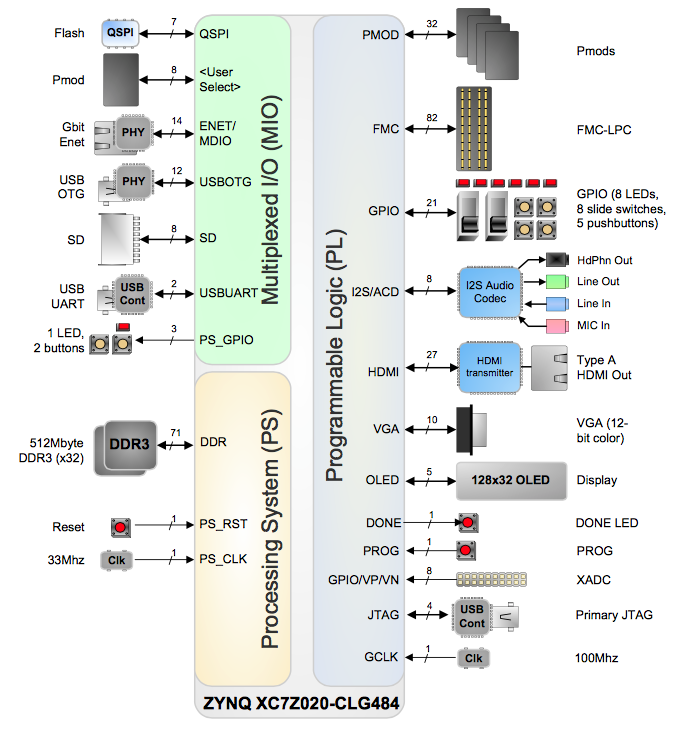
\includegraphics[width=0.85\textwidth]{ZedBoardBD.png}}
	\caption{ZedBoard Block Diagram \cite{zedboard_datasheet}}
	\label{zedboardbd}
\end{figure}
\par
As our research progressed, it became evident that FPGAs were a viable solution for implementing real-time situational awareness algorithms on a compact scale. For the purposes of this project, we decided to interface the ZedBoard with a stereo camera pair to gather disparity depth information on an area, and supplement that data with digital compass and rangefinder readings to produce detailed maps of the sensor suite's surroundings in real time. The implementation scheme for this device is detailed in the following chapter.





 %%%% Background %%%%
\newpage

\section{System Design}

\newpage
\section{System Implementation}
\subsection{Rangefinder Implementation}
With the data acquisition command tested and functioning properly, the rangefinder needs to be connected to the ZedBoard. Since the URG-04LX uses UART communication, there are a few reasonable options to create a UART controller on the ZedBoard.

\subsubsection{UART Options}
As the ZedBoard is such a powerful device, it has a few different options for controlling UART. A few of them are by controlling UART through linux, through a MicroBlaze soft-core processor, or through the Zynq-7000 Processing System. Running linux on the ZedBoard would use much of the board's valuable resources, and we would only be using a fraction of the capability provided by linux. The MicroBlaze soft-core processor would be a better alternative, but it runs in the programmable logic in the FPGA and is unnecessary when the ARM processor on the ZedBoard is unused \cite{microblaze}. Because of this, we decided to utilize the ARM processor on the ZedBoard by using the Zynq7 Processing System via Xilinx's Zynq-7000 Processing System Intellectual Property (IP) core.

\subsubsection{Zynq7 Processing System}
The ZedBoard SoC features a dual-core ARM Cortex-A9 MPCore processing system and Xilinx Programmable Logic. The Zynq7 Processing System IP core acts as a logic interface that integrates the Programmable Software (PS) with the Programmable Logic (PL), which allows access to both on-chip and external memory interfaces, to PL clocks, to many I/O peripherals, and even to extended I/O peripherals \cite{zynq7ps}. With all of this overwhelming functionality, the processing system is easy to customize, featuring a simple user interface, once it is added into a project's block design. The user interface can be used to change the processing system's activated features. Figure \ref{zynq7ps_pic} below shows the processing system customization window.

\begin{figure}[H]
	\centerline{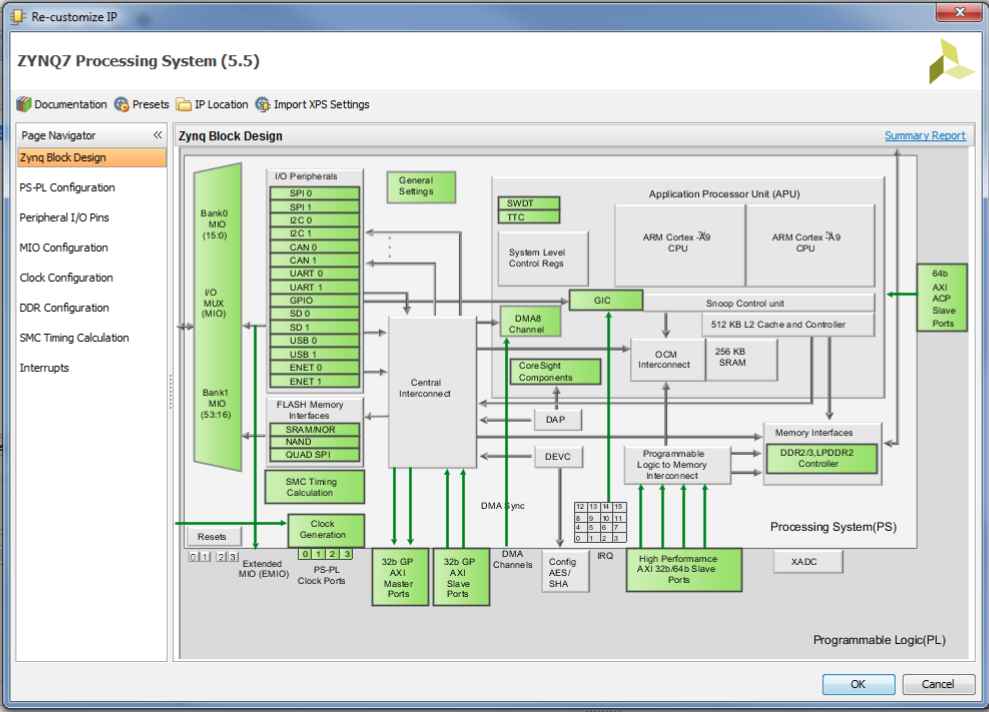
\includegraphics[width=1\textwidth]{zynq7ps.png}}
	\caption{Zynq7 Processing System Customization Window \cite{zynq7ps}}
	\label{zynq7ps_pic}
\end{figure}

In the figure above there are two options for UART shown: UART0 and UART1. The functionality of UART0 and UART1 are nearly identical, except that UART1 has the capability of being routed to the ZedBoard's USB UART port, which is not compatible with the rangefinder \cite{zedboard_datasheet}. So, we arbitrarily chose UART0 and routed the signals to MIO10 and MIO11, which correspond to the ZedBoard's PS Pmod, JE.
\par
After choosing UART0 and configuring the MIO pins, the Baud Rate needs to be configured such that it corresponds with the rangefinder's default communication speed, 19200 Baud \cite{urg04lx_datasheet}. This can be done in the processing system's customization window under PS-PL Configuration on the sidebar in Figure \ref{zynq7ps_pic}. Figure \ref{zynq7ps_baud_pic} below shows the PS-PL Configuration window.

\begin{figure}[H]
	\centerline{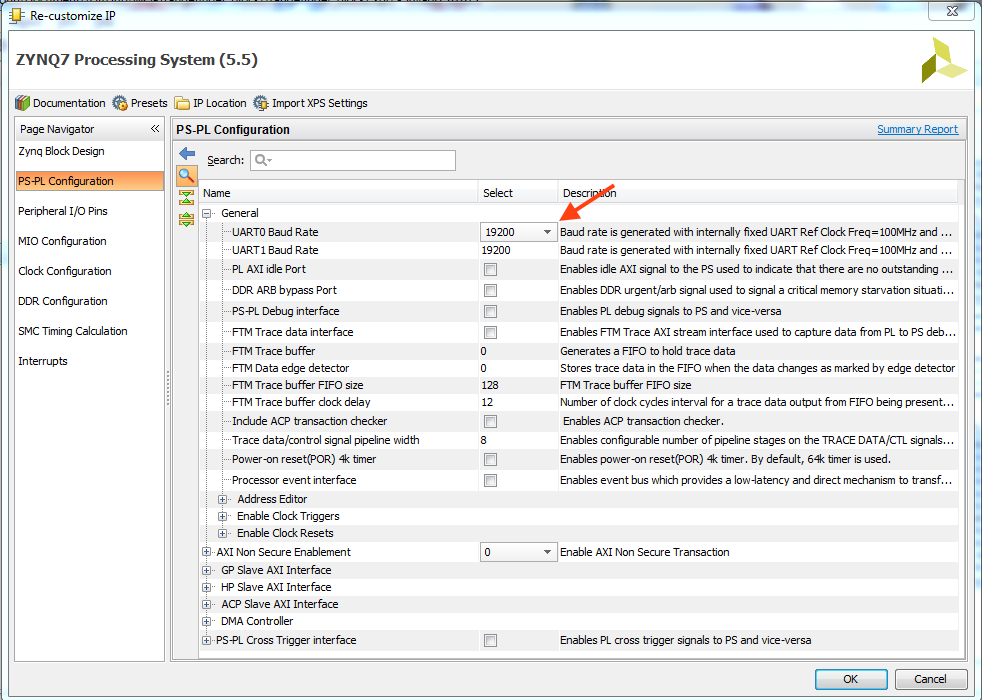
\includegraphics[width=1\textwidth]{zynq7ps_baud.png}}
	\caption{Zynq7 Processing System PS-PL Configuration Window}
	\label{zynq7ps_baud_pic}
\end{figure}

With the processing system customized in this fashion, the programmable logic's configuration is complete.

\subsubsection{PS-PL Communication / Creating Custom IP}
\label{sssec:ps_pl}
maybe break into two sections? one for ps-pl and talk about what AXI is and why we need to use it, and then in the testing and results section make a second one about how we needed to create custom axi peripherals? whatever works best
I HAVE NO IDEA WHAT TO WRITE FOR THIS

\newpage 
\section{Testing and Results}
\subsection{Camera Testing}
After obtaining two of the MT9V034 cameras chosen through the process referenced in Appendix item \ref{camdecision}, several steps were taken to obtain test images from each camera. These steps are outlined in the following sections.

\subsubsection{Camera Operation}
In order to gather working images from each camera module, we first needed to understand what circuitry our camera module breakouts contained so that we could interface with them. The MT9V034 camera breakouts used have been purchased through Leopard Imaging Inc. Although these camera module breakout boards are intended to be used with Leopard Imaging's LeopardBoard ARM development board, the breakouts were found to contain only the supporting circuitry recommended in the MT9V034 datasheet, and we decided that they would be ideal for our application \cite{livm34lp,mt9v034}. 
\par
Once the schematics of each camera module breakout were known, it was then possible to design a basic control interface for each camera. According to the MT9V034 datasheet, each camera module needs to be supplied with an external Master Clock and Output Enable signal in order to operate \cite{mt9v034}. A simple Verilog module for the Nexys3 Spartan-6 FPGA board was created in order to supply the camera module with a 24MHz master clock signal, and a switch was used to toggle output enable. With this module implemented, the camera module's default outputs could then be observed. In order to interface the camera module with an FPGA, the breakout board shown in Figure \ref{camBreakoutBoard} was also created to make the module's pins more easily accessible. 

\begin{figure}[H]
	\centerline{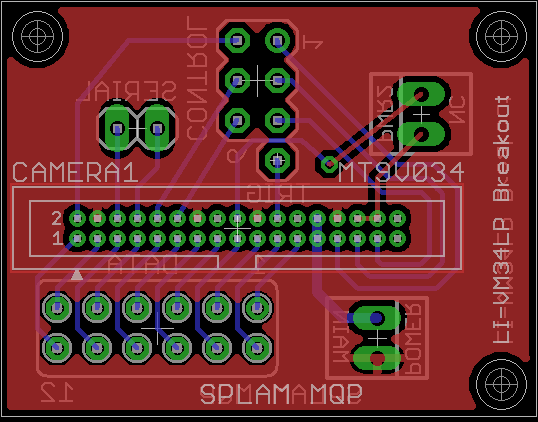
\includegraphics[width=0.5\textwidth]{camera_board.png}}
	\caption{LI-VM34LP Breakout Board}
	\label{camBreakoutBoard}
\end{figure}

\par
By default, the MT9V034 camera module will continuously gather image data at 60Hz  as long as it is supplied with an external clock signal and output is enabled \cite{mt9v034}. Several output signals from the camera module are then used to transmit image data. Each image, or frame, is broken up into individual "lines" which correspond to a line of pixels that stretch the width of the frame. Since our camera module captures images at 752x480 pixel resolution, one frame will contain 480 lines of 752 pixels each. The camera module breaks up image data by frame and line, and camera data pins FRAME\_VALID and LINE\_VALID are toggled to indicate the transmission of a frame or line. The timing diagram shown in Figure \ref{FvLv} shows the operation of these pins while transmitting an image.

\begin{figure}[H]
	\centerline{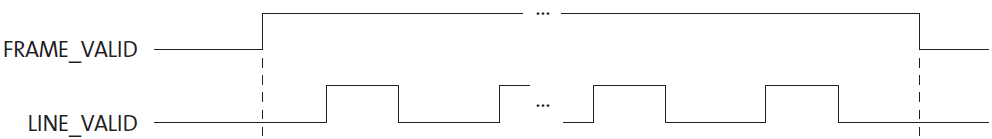
\includegraphics[width=1.0\textwidth]{camFvLv.png}}
	\caption{Frame and Line Valid \cite{mt9v034}}
	\label{FvLv}
\end{figure}

\par
Since the MT9V034 module transmits image data in parallel and each pixel contains 10 bits of resolution, 10 pins are used to transmit pixel values. Pixel data is transmitted in correspondence with LINE\_VALID and output clock signal PIXCLK. When LINE\_VALID is asserted, the pixel data pins are updated with values corresponding to pixels 0-751 of the given line. Values for each pixel are written out on the falling edge of the camera's PIXCLK pin, allowing for each pixel's value to be read on each rising PIXCLK edge. A full LINE\_VALID data transmission sequence will therefore contain 752 PIXCLK cycles, corresponding to the 752 pixels that make up the given line. A timing diagram of this data transmission scheme is shown in Figure \ref{LvDout}.  
\begin{figure}[H]
	\centerline{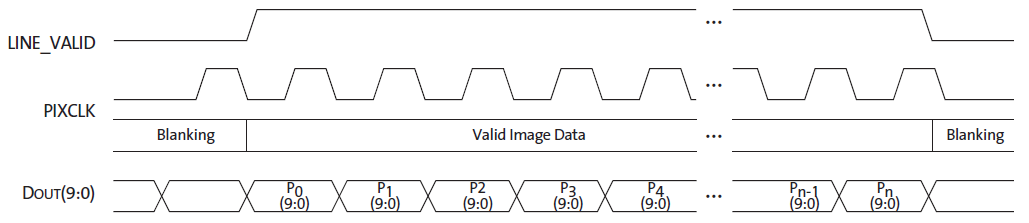
\includegraphics[width=1.0\textwidth]{camLvPckDout.png}}
	\caption{Line Data Transfer \cite{mt9v034}}
	\label{LvDout}
\end{figure}

\par
The default camera data transmission scheme was also examined using an oscilloscope, as shown in Figure \ref{camDataTransfer}, with channels 1-4 corresponding to camera PCLK, FRAME\_VALID, LINE\_VALID, and Data[0], respectively. In the case of Figure \ref{camDataTransfer}, the camera is initially powered off, resulting in an inactive PCLK signal during the beginning of the recording.
\begin{figure}[H]
	\centerline{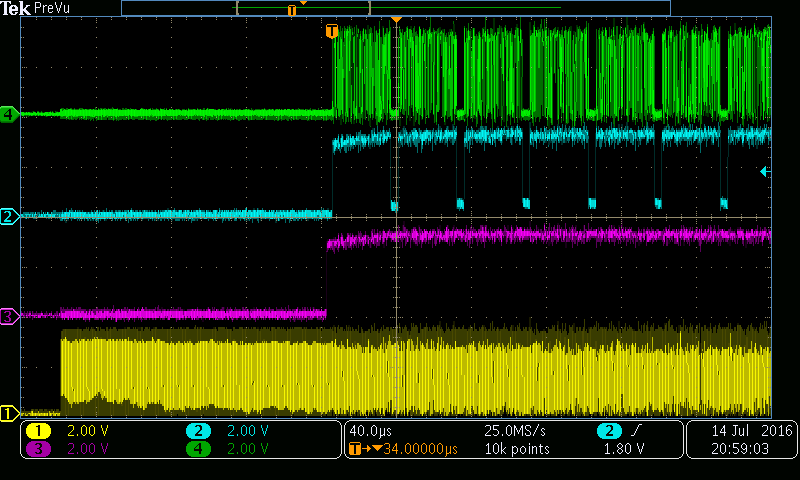
\includegraphics[width=1.0\textwidth]{oScope/pclk_fv_lv_data2/tek00004.png}}
	\caption{Camera Data Transfer}
	\label{camDataTransfer}
\end{figure}

\subsubsection{I$^2$C Control} 
The MT9V034 Camera module's mode of operation can be configured using a standard I$^2$C control interface. I$^2$C, or Inter-Integrated Circuit, is a bidirectional serial interface that allows for a master device to read from and write to several slave devices sharing the same data bus. An I$^2$C interface will use a Serial Data Line (SDA) and Serial Clock Line (SCL) that are normally pulled to 5V. When one connected I$^2$C device wishes to communicate with another, it will pull the SDA line low while leaving the SCL line high. The master device will then begin clocking the SCL line, and SDA will be used to transfer 7 bits representing the address of the desired slave device, along with an 8th bit representing whether it would like to read from or write to the device. An example of this transfer is shown in Figure \ref{I2Cexample}. A second 8 bit sequence representing a specific register within the slave device may also be transmitted following the device address. For example, if the master device wishes to write to slave device 0x40 at register 0x00, it will transmit 0x41 (address 0x40 and WRITE), followed by 0x00. If the slave device receives this transmission, it will acknowledge by pulling the SDA line low. At this point, the master can then transmit the value that it wishes to write to the given slave address and register. If the operation were a read rather than a write, the slave would transmit a value back to the master.  
\par
\begin{figure}[H]
	\centerline{
\includegraphics[width=1.0\textwidth]{I2C_data_transfer.png}}
	\caption{Example I$^2$C Data Transfer}
	\label{I2Cexample}
\end{figure}

Based on the LIVM34LP camera board schematic, each breakout board have been configured so that its camera is accessible at I$^2$C address 0x58 \cite{livm34lp,mt9v034}. Note that since both cameras come configured with the same I$^2$C bus address, a pullup resistor must be added to one of the cameras I$^2$C address lines so that both are individually accessible on a shared bus.
\par
Although the MT9V034 camera control registers are closed source, the previous model's registers are available in the camera module datasheet, and have been found to work with the current model thus far \cite{mt9v032}. As a baseline, the camera module was sent a read request at address 0x00, which should return 0x1324 for the MT9V034 camera module. An oscilloscope screenshot of this request is shown in Figure \ref{camVersion}, with the first packet consisting of a request to address 0x00 of device 0x058, and the second packet consisting of the camera's response of 0x1324. 
\begin{figure}[H]
	\centerline{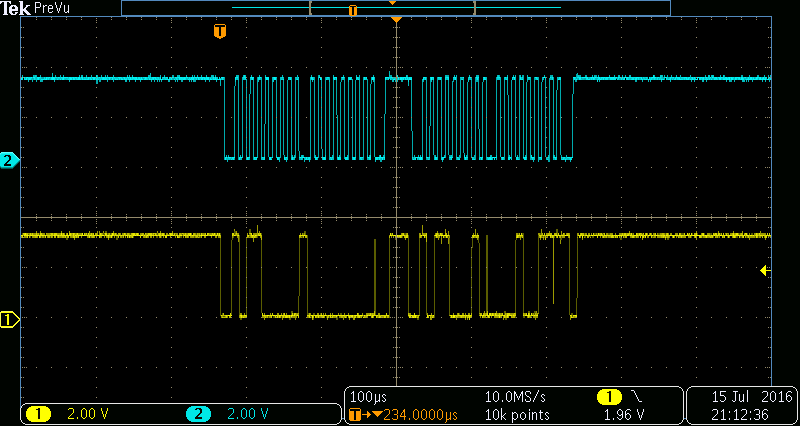
\includegraphics[width=1.0\textwidth]{oScope/i2c_0x00/tek00001.png}}
	\caption{Example I$^2$C Transfer with Camera}
	\label{camVersion}
\end{figure}

\par
After the camera I$^2$C was deemed working, the camera control register was modified to put the camera in "snapshot" mode. In this mode, the camera module will no longer continuously take pictures, and will only gather new images when an external trigger is activated. This is the mode that each camera will need to operate in in order to acquire stereo imagery, since a shared trigger line will allow for both cameras to be controlled simultaneously.
\par
According to the previous camera iteration's datasheet, the camera module's operational mode can be set through control register 0x07. By default, this register will be set to a value of 0x0388, which corresponds to master mode with parallel output and simultaneous readout of pixel data enabled \cite{mt9v032}. In order to put the camera in trigger mode, the control register needs to be written with value 0x0198, which allows for the same functionality as before with the exception of having continuous shutter mode replaced with an external trigger. For reference, a table with bit descriptions for the camera control register can be found in Appendix item \ref{camctlreg} \cite{mt9v032}.
\par
After modifying the state of this register, a button was attached to the camera's TRIGGER input line, and the TRIGGER and FRAME\_VALID lines were observed on channels one and two of the oscilloscope, as shown in Figure \ref{camInTrigMode}. This oscilloscope screenshot can be seen as an example of how the camera is no longer in continuous operation, since FRAME\_VALID only asserts itself in response to a TRIGGER input. 
\begin{figure}[H]
	\centerline{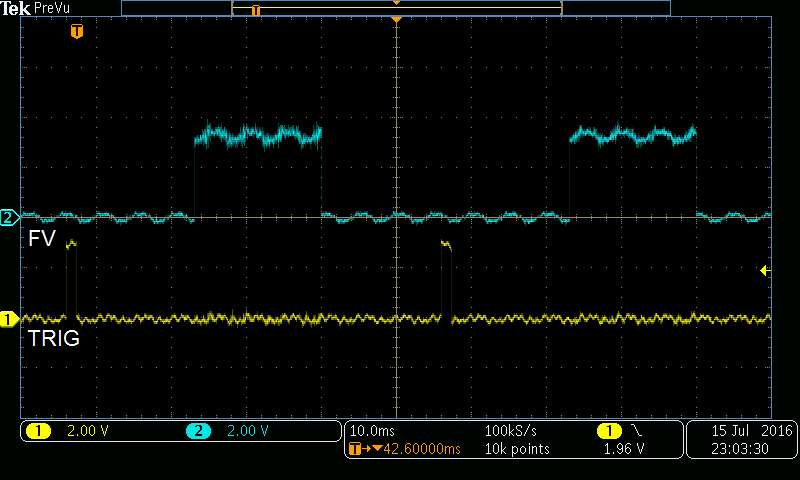
\includegraphics[width=1.0\textwidth]{oScope/i2c_0x07/externalTrigger/externalTrig.png}}
	\caption{Camera Trigger and FV in Trigger Mode}
	\label{camInTrigMode}
\end{figure}

\subsubsection{Data Management}
After successfully creating a camera control interface and placing the MT9V034 camera module in trigger mode, it was then possible to begin viewing images from the module. Since each image contains 752x480 pixels with 10 bits of resolution per pixel, a full camera image will consume 3,609,600 bits, or 440.6kB, as shown in Equation \ref{imagesize}.
\begin{equation} \label{imagesize}
Image\,\,Size = 752px*480px*10\frac{bits}{pixel} = 3609600\,bits*\frac{1\,byte}{8\,bits}*\frac{1 kB}{1024\,bytes} = 440.625kB
\end{equation}
\par
In order to send a camera image to a computer or monitor for viewing, several steps need to be taken. Although it would be ideal to transfer the image directly from the camera to a computer or display, this would be difficult to achieve due to the high speeds of the camera's data output. In order to properly synchronize camera data with a VGA display, both the camera and VGA display would have to run at exactly the same clock speed, and would need to have the same amount of vertical and horizontal blanking to display each pixel in its correct location. If the image were transferred to a computer, the act of packaging the information so that it may be interpreted by said computer would place severe limitations on the speed of the system. A proper solution to these timing issues would be to buffer the image between the camera and the desired output source, since this would allow for separate clock domains to be used for camera data transfer and data output. However, the act of locally buffering a camera image on an FPGA would also be difficult due to low memory resources. 
\par
Although 440kB may seem like a relatively small image size, creating a buffer object large enough for storing said image would consume an extremely large amount of logic. For reference, a standard Nexys3 FPGA evaluation board contains only 18kB of onboard Block RAM (internal memory), and would not be able to buffer an image of this size without the use of external memory\footnote{Xilinx, \textit{Spartan-6 FPGA Block RAM Resources}, 11.\\  \url{http://www.xilinx.com/support/documentation/user_guides/ug383.pdf}}. This leaves the final option of using either external memory or a First-In First-Out (FIFO) memory array for transferring a captured image between clock domains. During initial development, an AL422B FIFO IC was used, since the IC has been created specifically for buffering VGA imagery similar to that of the MT9V034 camera module, and can be connected directly to the camera module outputs \cite{al422b}. The AL422B FIFO module contains 3M-bits of RAM that can be written to and read from in parallel, and supports separate input and output clock speeds between 1-50MHz \cite{al422b}. This means that the camera module can write pixel data to the FIFO as long as it operates at a speed between 1 and 50MHz, and the FPGA can independently read from the FIFO at any speed within the same range. Note that since this FIFO supports only 8-bit parallel data in and out, the lowest two bits of camera pixel data must be truncated. This isn't a major issue, since the truncation will correspond to a 4/1024 reduction in the range of values that each pixel can map to.
\par
With the inclusion of the external FIFO module, it is now possible to capture and store an image for future reading, and to read out image data in chunks. Keeping this in mind, the system shown in Figure \ref{camTestBDG} was created for capturing, storing, and transmitting camera images to a computer for external analysis. In order to reduce development time, an external microcontroller was used for controlling the camera module's I$^2$C interface and placing the module in trigger mode. Various buttons and switches on the FPGA were then used for controlling the camera output and trigger, allowing for a user to trigger an image for storage on the AL422B FIFO. Once the image has been stored on the FIFO, the FPGA is capable of reading the image line-by-line into an internal buffer. An internal System on Chip (SoC) is used to control FPGA reads from the FIFO into this internal buffer. An image dump will begin when the SoC microcontroller signals to the FPGA to read a new line of pixels into its internal 8 bit by 752 address pixel buffer. The FPGA will then signal to the microcontroller when this buffer has been filled, and the microcontroller will print out the value of each pixel in the buffer to a connected computer over a Universal Asynchronous Reciever/Transmitter (UART) port. When the microcontroller finishes printing out the value of each pixel in the line buffer, it will signal to the FPGA to read in a new line of pixels. This process will repeat for each of the 480 lines of pixels in the image, allowing for the transmission of an entire image's worth of data from FIFO to computer. The Verilog implementation of the top module and line buffer for this interface can be found in Appendix item \ref{mt9v034TestCode}.

\begin{figure}[H]
	\centerline{\includegraphics[width=1.2\textwidth]{camTestBlockDiag.png}}
	\caption{Camera Test System Block Diagram}
	\label{camTestBDG}
\end{figure}
\par
An example of the transmission of one line of pixel data from the FIFO to the FPGA is shown in Figure \ref{fifoDataOut}.  The green, purple, blue, and yellow lines in this image represent pixel data, FIFO read enable, read reset, and read clock, respectively. Since the FPGA reads in one line of pixel data at a time, this process will take 752 read clock cycles, as measured in Figure \ref{fifoDataOut}. In order to simplify debugging, an internal counter and seven-segment display controller have also been implemented on the FPGA, and will display a running count of the number of pixel lines that have been read into the FPGA's internal buffer, ranging from 0x0000-0x01E0 (0-480). 
\begin{figure}[H]
	\centerline{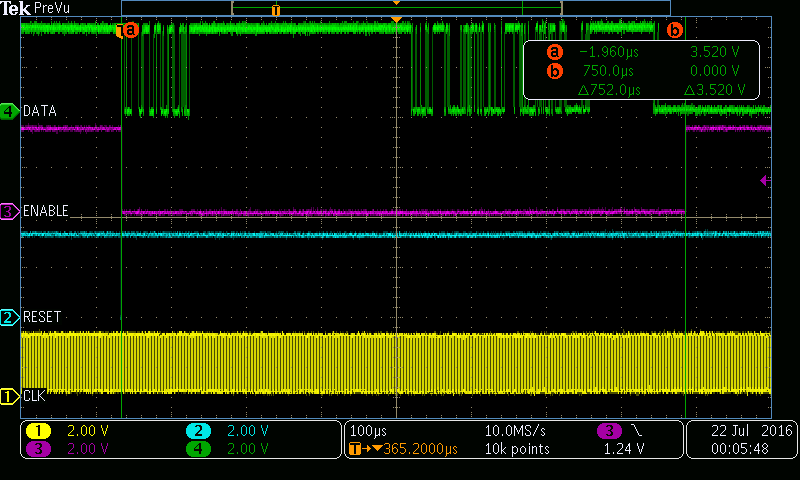
\includegraphics[width=1.0\textwidth]{oScope/camera_fifo/fifo_rstAndDataTimed.png}}
	\caption{Transferring Line Data from FIFO to FPGA}
	\label{fifoDataOut}
\end{figure}

\subsubsection{Transmitting Images Over UART for Analysis}
Once the FIFO and FPGA line buffer interfaces were created, the source code found in Appendix item \ref{camTestC} was implemented on a Microblaze SoC in order to transmit camera line data from the FPGA's internal line buffer over UART. An example of the microcontroller's UART output is shown in Figure \ref{PuTTYfifoData}. The microcontroller will print the value of each pixel followed by a newline and carriage return, starting with the top left pixel in the acquired image. 
\begin{figure}[H]
	\centerline{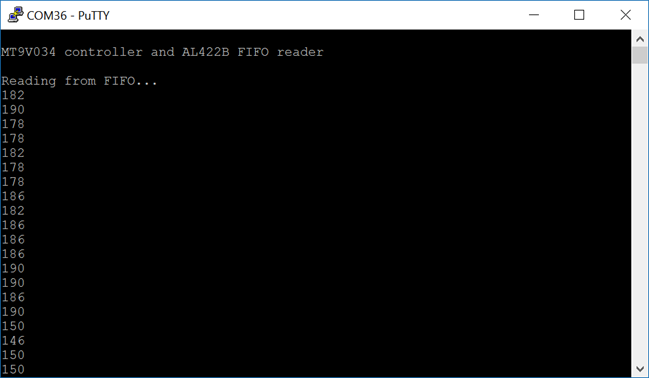
\includegraphics[width=0.8\textwidth]{oScope/camera_fifo/PuTTy.png}}
	\caption{Reading FIFO Data}
	\label{PuTTYfifoData}
\end{figure}
\par
After the image is received through PuTTy, the \textsc{Matlab} script found in Appendix item \ref{camTestMatlab} is used to parse the corresponding logfile into a greyscale image. An example image created through this process is shown in Figure \ref{notebookImage}. Note that the sub-optimal quality of this image is due to signal interference and degradation in the test setup's long wiring, as shown in Figure \ref{camTestSetup}. 
\begin{figure}[H]
	\centerline{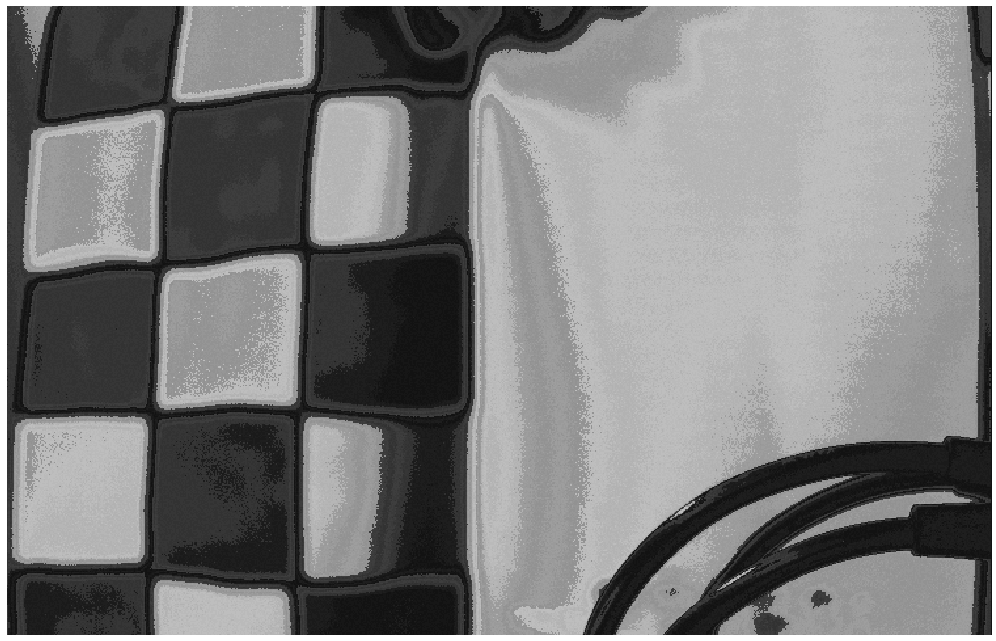
\includegraphics[width=0.75\textwidth]{oScope/camera_fifo/notebook.png}}
	\caption{Notebook With Grid and Oscilloscope Leads}
	\label{notebookImage}
\end{figure}
\par
Although this system was tested using the Nexys3 (Spartan-6) FPGA board, the use of an external FIFO and little to no platform-specific hardware make it so that it can easily be implemented on any system, including the Zynq family of processors that we will be implementing our final system on.   
\begin{figure}[H]
	\centerline{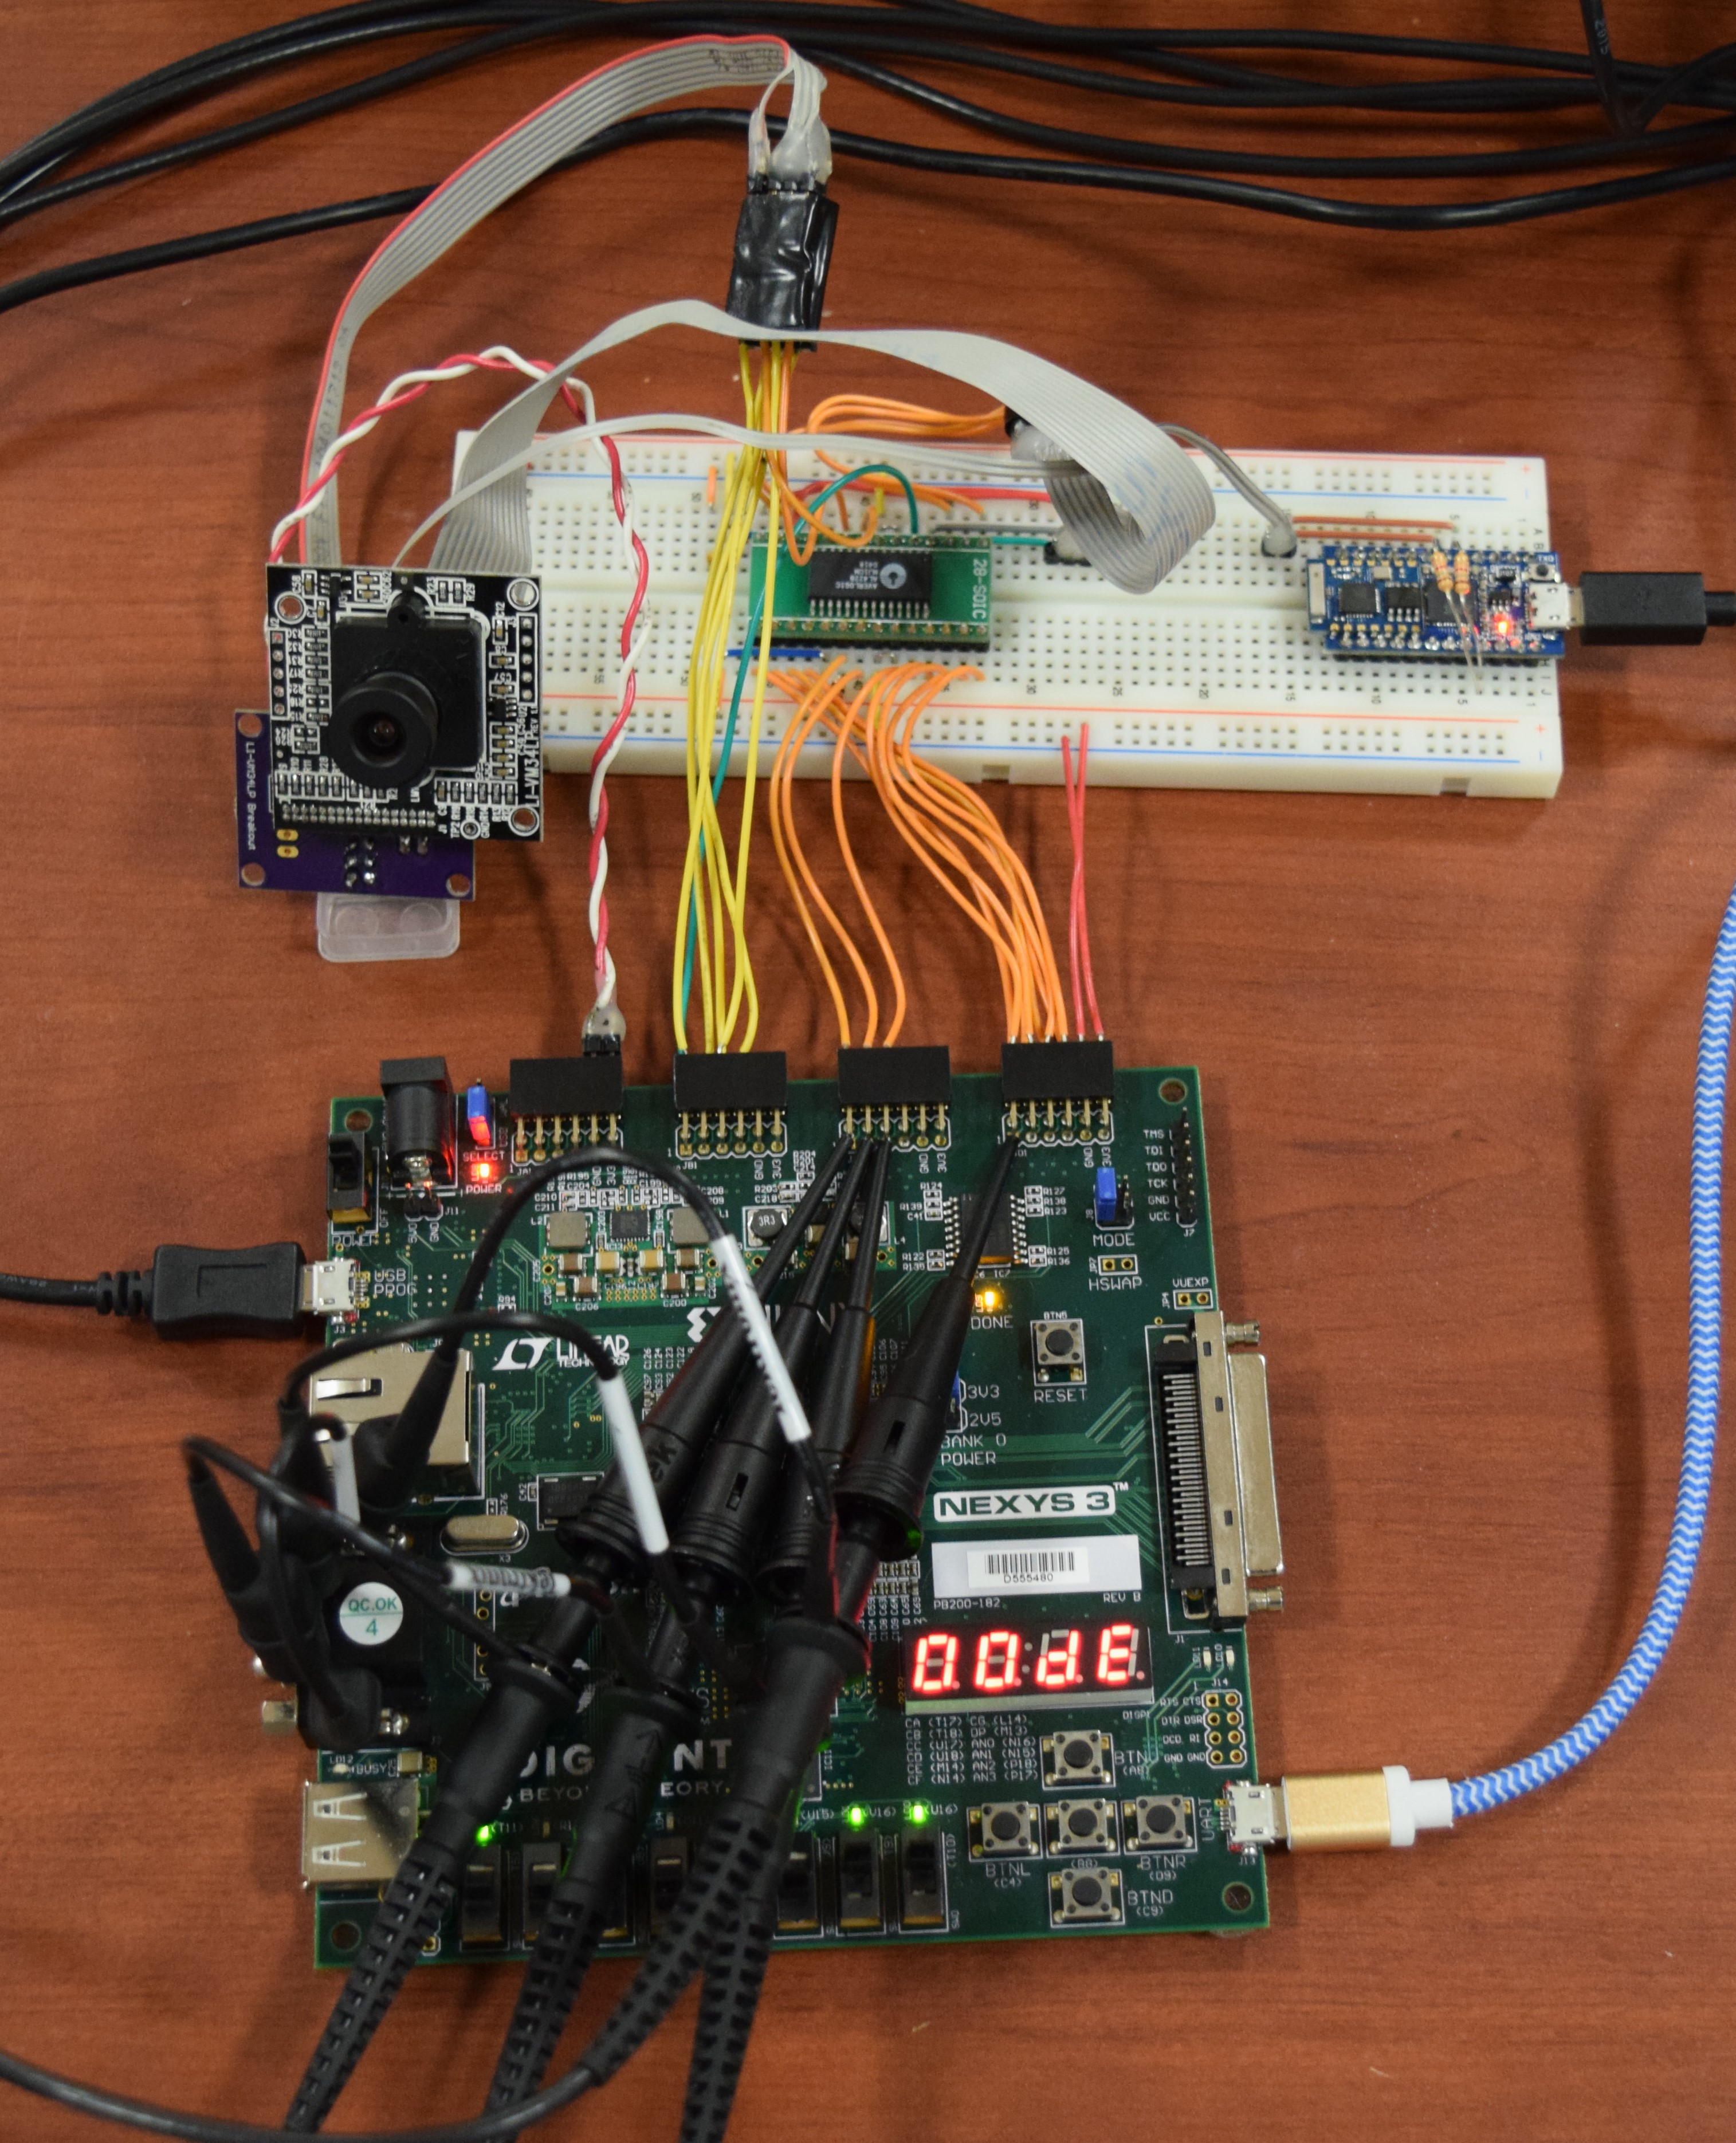
\includegraphics[width=0.75\textwidth]{oScope/camera_fifo/camTestSetup.jpg}}
	\caption{Camera Test Setup}
	\label{camTestSetup}
\end{figure}

\subsection{Disparity Algorithm}
After verifying that the camera interface was functional, a large portion of time was spent implementing a disparity algorithm that would allow for the extraction of 3D depth information from stereo image data. This algorithm was first implemented in \textsc{Matlab}, and was then transferred to programmable logic after the algorithm was verified working. 
\subsubsection{Sum of Absolute Differences}
The method used in our disparity algorithm implementation is known as the Sum of Absolute Differences, or SAD. SAD is a common digital image processing technique used to measure the similarity between blocks of image data. In the case of our stereo camera interface, a SAD algorithm is used to search through the right image data for windowed blocks that match a template block selected from the left camera image. This process is performed using 7x7 pixel search blocks over 50 pixel horizontal ranges, and is repeated throughout the image. The expression for the sum of absolute differences is shown in Equation \ref{disparityEQN} below. 
\par
% sum(sum(abs(template-block)))
\begin{equation}\label{disparityEQN}
SAD = \sum_{x}^{}\sum_{y}^{}|template-block|
\end{equation}
\par
A visual representation of the Sum of Absolute differences is shown in Figure \ref{SAD}, with the top image showing the left image template block, and the middle image showing the right image search window in relation to the location of the template block. Below both images is a visual representation of the Sum of Absolute Differences between the template block and the current search block, outlined in white. In the case of the current search, the template and search blocks are relatively different, resulting in a high SAD value. 
\par
\begin{figure}[H]
	\centerline{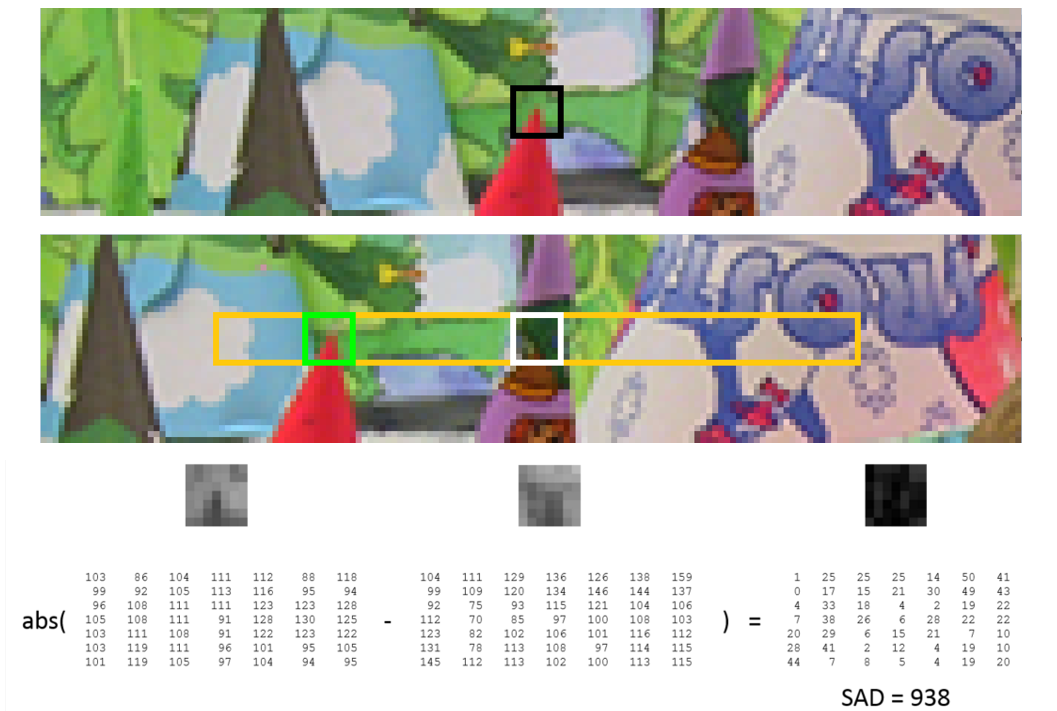
\includegraphics[width=0.75\textwidth]{SAD.PNG}}
	\caption{Sum of Absolute Differences \cite{mccormick}}
	\label{SAD}
\end{figure}
\par
Since the disparity algorithm used in this implementation calculates the sum of absolute differences for multiple search blocks, the resulting SAD values for each search block can be compared to find the location of the most similar matching block in the search image. Due to the nature of the SAD algorithm, lower SAD values indicate higher similarity between the template and search blocks. This comparison is demonstrated in Figure \ref{blockMatching} below. In the case of Figure 
ref{blockMatching}, higher match score values for each search block indicate lower SAD values.
\par
\begin{figure}[H]
	\centerline{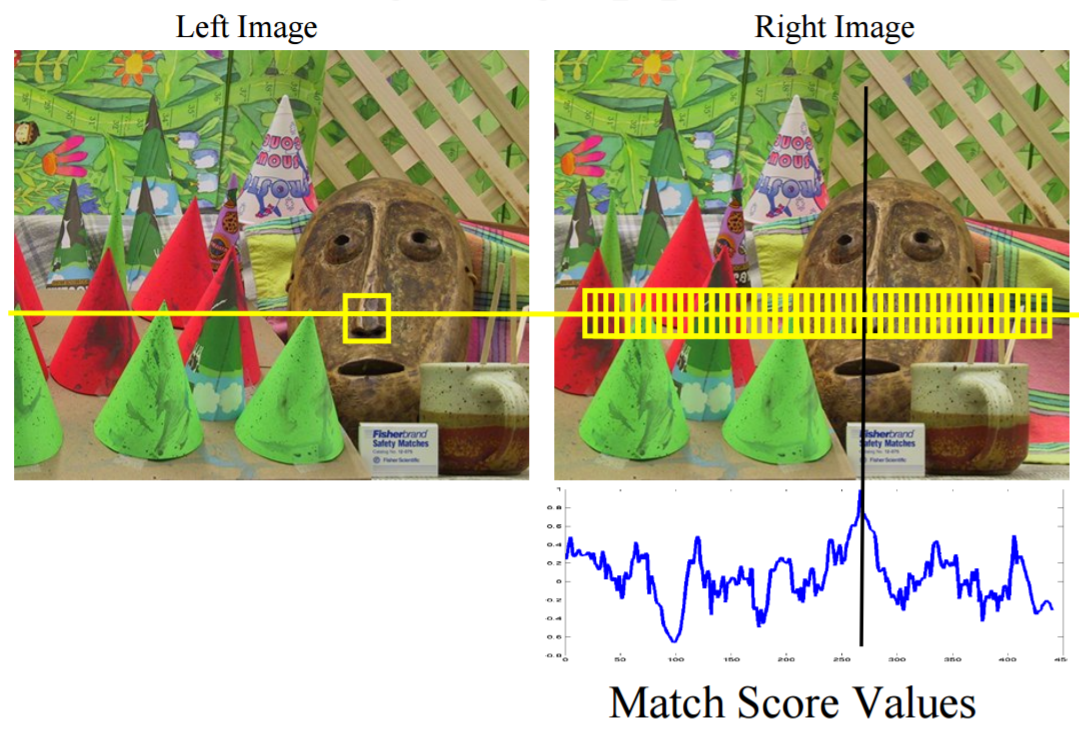
\includegraphics[width=0.75\textwidth]{blockMatching.PNG}}
	\caption{Block Matching Overview \cite{collins}}
	\label{blockMatching}
\end{figure}
\par
The SAD at multiple search points can be used to estimate the pixel offset between the template block and matching search block based on array index locations, since all SAD values for a single search are stored in a vector. This pixel offset is known as the disparity value for a given template and search block. The disparity $d$ at a given point can be transformed into a units of distance using the focal point $f$ and baseline distance $T_x$ between image sensors as shown in Equation \ref{disp2dist} below. 
\par
\begin{equation}\label{disp2dist}
depth = Z = \frac{fT_x}{d}
\end{equation}
\par
Pixel coloration values in a disparity image are based on the distance calculation shown in Equation \ref{disp2dist}, where each pixel is referenced to the disparity at a given template block's location. An example disparity image created using the \textsc{Matlab} code found in Appendix item \ref{disparityTestMatlab} is shown in Figure \ref{disparityOutput} below. 
\par
\begin{figure}[H]
	\centerline{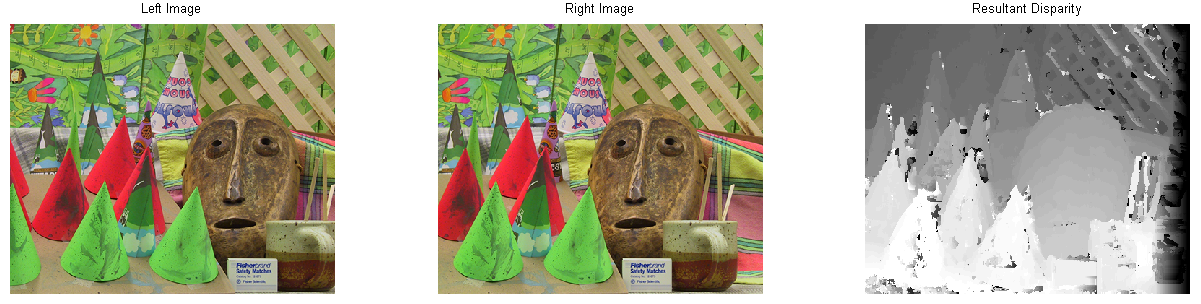
\includegraphics[width=1.1\textwidth]{disparity.png}}
	\caption{Disparity Algorithm Output}
	\label{disparityOutput}
\end{figure}

\subsubsection{Image Rectification}
The Sum of Absolute Differences algorithm operates under the assumption that objects in both camera images lie on the same horizontal line between both images, known as an epipolar line. An example of shared epipolar lines between camera imagery is shown in Figure \ref{epipolarLines} below. Although an ideal stereo camera setup would contain shared epipolar lines between camera images, raw image data from each camera will contain slight differences in object location based on the physical position of the camera modules, as well as minor differences in the lenses of each camera. Both input images can be adjusted to share the same epipolar lines through a post-processing step known as image rectification. 
\par
\begin{figure}[H]
	\centerline{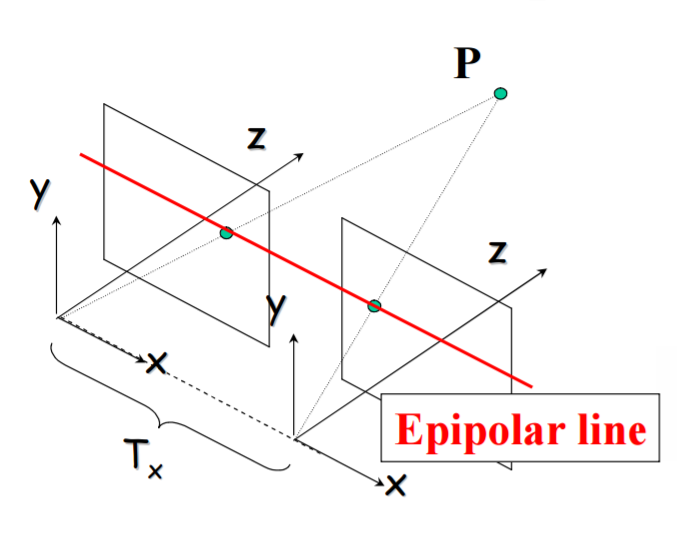
\includegraphics[width=0.75\textwidth]{epipolarLines.PNG}}
	\caption{Horizontal Epipolar Lines \cite{collins}}
	\label{epipolarLines}
\end{figure}
\par
A pictorial representation of the process of stereo image rectification is shown in Figure \ref{rectification} below \cite{mattoccia_slides}. This process is achieved using a 3x3 matrix coordinate transform based on parameters obtained from the external calibration process. 
\begin{figure}[H]
	\centerline{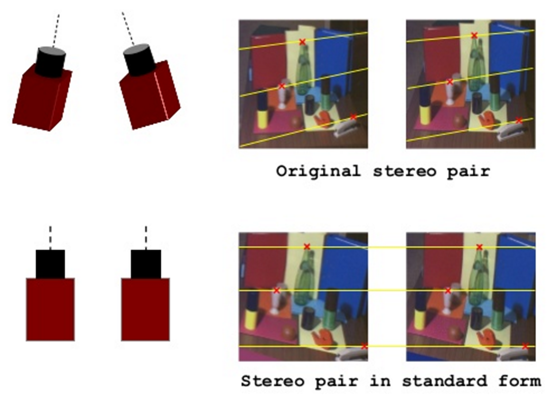
\includegraphics[width=0.75\textwidth]{rectification.png}}
	\caption{Stereo Image Rectification \cite{mattoccia_slides}}
	\label{rectification}
\end{figure}
\par
ADD AN EXAMPLE OF THE MATLAB CALIBRATION STUFF (figures showing 3d anaglyph process)

\subsubsection{Test Implementation}
The original disparity test implementation used closely follows the \textsc{Matlab} disparity algorithm shown in Appendix item \ref{disparityTestMatlab}. This algorithm is implemented using a finite state machine with five states, as shown in Figure \ref{disparityTestImp} below. In order to maintain simplicity, the test algorithm has been implemented to operate on 46x30 windowed portions of the input imagery. By default, the disparity module will remain in an idle state until an external enable signal is toggled high using a button input. This will cause the finite state machine to advance to its READ state, and image data for the left and right camera images will be read in from the stereo camera breakout board. After image data has been received, the state machine will then advance to a cyclical set of states used for iterating through each image and calculating disparity. 
\par
The disparity module will begin by isolating the template and search blocks from the right and left image data in the finite state machine's separation state. Next, the state machine will advance to its SAD state, and will calculate the sum of absolute differences between the template and search block. This value is placed in a vector that matches the length of the search range. If the vector hasn't been completely filled, indicating that there are more search blocks to compare to the template, the state machine will revert back to the separate state, isolating a new search block from the right camera image. When the SAD vector is full, the state machine will advance to its finalization state. 
\par
\begin{figure}[H]
	\centerline{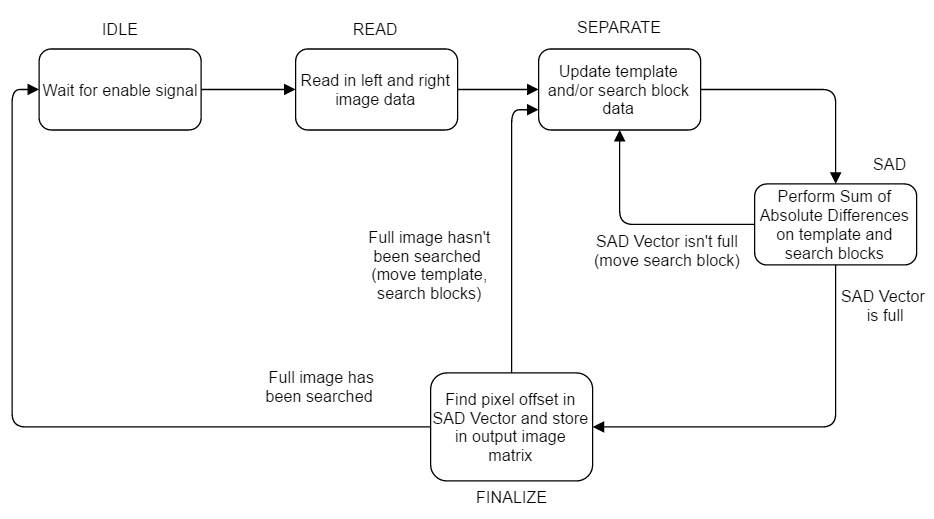
\includegraphics[width=0.75\textwidth]{looping_disparity.png}}
	\caption{Disparity Test Implementation}
	\label{disparityTestImp}
\end{figure}
\par
The finalization state is used to search through the SAD vector for the lowest value. The index of this value within the SAD vector in reference to the template block location is used to create a disparity value for the given template block location. This value is then converted to a distance using Equation \ref{disp2dist}, and is stored in the output image location. If the output image hasn't been fully populated with distance values, the state machine will then revert back to the separate state. Otherwise, the state machine will advance to its idle state, and the resulting disparity image can be read for output. 
\par
This module was initially tested using a verilog test bench, and was then tested using camera image data and a VGA display controller module, allowing for real-time verification of the algorithm's effectiveness. After testing the initial disparity algorithm, several modifications were made to increase the overall speed and efficiency of the disparity module. 

\subsubsection{Final Implementation}
\begin{figure}[H]
	\centerline{\includegraphics[width=1.2\textwidth]{Disparity_Algorithm.png}}
	\caption{Disparity Final Implementation}
	\label{disparityTestImp}
\end{figure}


\newpage 
\section{Conclusions}

\newpage
\singlespacing
%https://www.sharelatex.com/learn/Bibliography_management_with_bibtex
\begin{thebibliography}{9}

\bibitem{al422b}
Averlogic.
\textit{AL422B Data Sheets}. 2001.
Available from: \url{http://www.frc.ri.cmu.edu/projects/buzzard/mve/HWSpecs-1/Documentation/AL422B_Data_Sheets.pdf}.

\bibitem{davison} 
Davison, A.J.,
\textit{Real-Time Simultaneous Localisation and Mapping with a Single Camera}. 
IEEE Computer Vision, 2003. 2(1).

\bibitem{livm34lp}
Leopard Imaging Inc.
\textit{LI-VM34LP Camera Board}. 2009.
Available from: \url{http://www.leopardimaging.com/uploads/li-vm34lp_v1.1.pdf}.

\bibitem{serveball}
\textit{Serveball}.
Available from: \url{http://www.serveball.com/}.

\bibitem{mattoccia}
Stefano Mattoccia, M.P.,
\textit{A passive RGBD sensor for accurate and real-time depth sensing self-contained into an FPGA}.
in \textit{International Conference on Distributed Smart Cameras}. 2015.

\bibitem{mt9v032}
On Semiconductor. 
\textit{MT9V032: 1/3-Inch Wide-VGA CMOS Digital Image Sensor}. 2015. 
Available from: \url{http://www.onsemi.com/pub_link/Collateral/MT9V032-D.PDF}.

\bibitem{mt9v034}
On Semiconductor. 
\textit{MT9V034: 1/3-Inch Wide-VGA CMOS Digital Image Sensor}. 2015. 
Available from: \url{http://www.onsemi.com/pub_link/Collateral/MT9V034-D.PDF}.

\bibitem{porikli}
Fatih Porikli, O.T.,
\textit{Human Body Tracking by Adaptive Background Models and Mean-Shift Analysis}.
in \textit{IEEE International Workshop on Performance Evaluation of Tracking and Surveillance}. 2003.

\bibitem{thrun}
Sebastian Thrun, D.H., David Ferguson, Michael Montemerlo, Rudolph Triebel, and C.B. Wolfram Burgard, Zachary Omohundro, Scott Thayer, William Whittaker.
\textit{A System for Volumetric Robotic Mapping of Abandoned Mines}. 
in \textit{IEEE International Conference on Robotics and Automation}. 2003.

\end{thebibliography}

% include in ToC - must be after refs for correct page link from hyper
\addcontentsline{toc}{section}{References} %%%% Bibliography %%%%
\doublespacing
\newpage

\section{Appendix} %%%% Appendix %%%% 
\subsection{Useful Resources}
This section is intended to serve as complete compilation of all resources gathered throughout D Term 2016 that we believe will be useful as we begin to work on the methodology portion of our project.

\begin{itemize}
  \item Strother, Daniel. 2011. "Open-Source FPGA Stereo Vision Core Released." \path{https://danstrother.com/2011/06/10/fpga-stereo-vision-core-released/}.
  
  \item Field, Mike. 2013. "Zedboard OV7670." \path{http://hamsterworks.co.nz/mediawiki/index.php/Zedboard_OV7670}.
  
  \item "OV7670/OV7671 CMOS VGA CameraChip Implementation Guide." \path{https://www.fer.unizg.hr/_download/repository/OV7670new.pdf}.
  
  \item "MIPI CSI2-to-CMOS Parallel Sensor Bridge - Lattice Semiconductor." \path{http://www.latticesemi.com/~/media/LatticeSemi/Documents/ReferenceDesigns/JM/MIPICSI2to CMOSParallelSensorBridgeDocumentation.pdf?document_id=50533}.
  
  \item "OmniVision Serial Camera Control Bus (SCCB) Functional Specification." \path{http://www.ovt.com/download_document.php?type=document&DID=63"}.
  
  \item Morvan, Yannick. "Multiple-View Depth Estimation." \path{http://www.epixea.com/research/multi-view-coding-thesisse15.html}.
  
  \item MathWorks. "Depth Estimation From Stereo Video." \path{http://www.mathworks.com/help/vision/examples/depth-estimation-from-stereo-video.html}.
  
  \item Stefano Mattoccia, Matteo Poggi. 2015. "A passive RGBD sensor for accurate and real-time depth sensing self-contained into an FPGA". International Conference on Distributed Smart Cameras.
  
  \item Mattoccia, Stefano. 2013. "Stereo Vision: Algorithms and Applications." \path{http://www.slideshare.net/DngNguyn43/stereo-vision-42147593}.
  
  \item Szeliski, Richard. 2010. Computer Vision: Algorithms and Applications. New York: Springer.
  
  \item Beau Tippets, Dah Jye Lee, Kirt Lillywhite, James Archibald. 2013. "Review of Stereo Vision Algorithms and Their Suitability for Resource-Limited Systems." Journal of Real-Time Image Processing 11 (1). doi: 10.1007/s11554-012-0313-2.
  
  \item Jouni Rantakokko, Joakim Rydell, Peter Stromback, Peter Handel, Jonas Callmer, David Tornqvist, Fredrik Gustafsson, Magnus Jobs, Mathias Gruden. 2011. "Accurate and Reliable Soldier and First Responder Indoor Positioning: Multisensor Systems and Cooperative Localization." IEEE Wireless Communications 18 (2):10-18. doi: 10.1109/MWC.2011.5751291.
  
  \item Davison, Andrew J. 2003. "Real-Time Simultaneous Localisation and Mapping with a Single Camera."  IEEE Computer Vision 2 (1). doi: 10.1109/ICCV.2003.1238654.
  
  \item Fatih Porikli, Oncel Tuzel. 2003. "Human Body Tracking by Adaptive Background Models and Mean-Shift Analysis." IEEE International Workshop on Performance Evaluation of Tracking and Surveillance.
  
  \item Giovanni Pintore, Enrico Gobbetti. "Effective mobile mapping of multi-room indoor structures."  The Visual Computer 30 (6):707-716. doi: 10.1007/s00371-014-0947-0.
  
  \item "iRobot 110 FirstLook." iRobot. \path{http://www.irobot.com/$~$/media/Files/Robots/Defense/FirstLook/iRobot-110-FirstLook-Specs.pdf}.

\end{itemize}
 % useful resources
\subsection{Component Selection} \label{componentSelection}

\begin{center}
\begin{tabular}{ |c|c|c|c| } 
 \hline
 \textbf{Component} & \textbf{Part Number}  & \textbf{Supplier} & \textbf{Cost}  \\ \hline
 FPGA & ZedBoard & Borrowed & N/A  \\ \hline
 IMU & PmodNav & Digilent & \$45  \\ \hline
 Rangefinder & URG-04LX & Borrowed & N/A  \\ \hline
 RS232 to TTL Converter & MAX232CSE & uxcell & \$7  \\ \hline
 RS232 Breakout Board & Swellder DB9 & VIKINS Tech & \$7  \\ \hline
 Stereo Cameras$^\dagger$ & MT9V034 & Mouser & \$146  \\ 
 \hline
\end{tabular}
\end{center}
$^\dagger$ Note that we originally planned to purchase a flir lepton thermal camera module and accompanying breakout board to support two stereo ov7670 camera modules. After experimenting with the ov7670 camera module on our FPGA board, we began to realize that these camera modules are highly limited due to their low frame rate and poor documentation, and realized that we wanted to search for a different camera module. In addition, at a price of \$223 for a thermal camera with an 80x60 degree resolution, 25 degree fov, and 7-9Hz image sample rate, we believe that we are much better off spending our money on better camera modules that will be more usable for our task. For more information see Section  \ref{camdecision}. % component selection
\subsection{Camera Module Decision Matrix}
\singlespacing
\begin{small}
\centerline{
\begin{tabular}{ |L{2cm}|L{1.5cm}|L{2.5cm}|L{1cm}|L{1.7cm}|L{2cm}|L{1.7cm}|L{1.2cm}|L{1cm}| } 
 \hline
 \textbf{Camera Module} & \textbf{Max Frame Rate (FPS)}  & \textbf{Resolution at Max Frame Rate (px.)} & \textbf{Cost} & \textbf{Requires External Adapter} & \textbf{Data Transfer Interface} & \textbf{Shutter} & \textbf{Field of View (deg.)} & \textbf{Rank 0-10}  \\ \hline
 OV7670 & \cellcolor{red!25} 30 & \cellcolor{green!25} 640x480 & \cellcolor{green!50} \$10 & \cellcolor{green!25} No & \cellcolor{green!25} Parallel & \cellcolor{red!25} Rolling & \cellcolor{red!25}  25 & 5  \\ \hline
 Raspberry Pi Camera &\cellcolor{green!25}  90 & \cellcolor{green!25} 640x480 & \cellcolor{green!25}  \$30 & \cellcolor{red!25} Yes, \$53 & \cellcolor{red!25} MIPI (CSI2) & \cellcolor{red!25}  Rolling & \cellcolor{green!25} 49 & 6  \\  \hline
 PC1089K & \cellcolor{green!25} 60 & \cellcolor{green!25} 720x480 & \cellcolor{green!25} \$32 & \cellcolor{green!25} No & \cellcolor{red!50} NSTC/ PAL & \cellcolor{red!25} Rolling & Not Given & 5 \\ \hline 
 OV4682 & \cellcolor{green!50} 330 & \cellcolor{green!25} 640x480 & \cellcolor{red!25} \$89 & \cellcolor{red!25} Yes, \$50 & \cellcolor{red!25} MIPI & \cellcolor{red!25} Rolling & Not Given & 6 \\ \hline
 \textbf{MT9V034} & \cellcolor{green!25} \textbf{60} & \cellcolor{green!25} \textbf{750x480} & \cellcolor{red!25} \textbf{\$73} & \cellcolor{green!25} \textbf{No} & \cellcolor{green!25} \textbf{Parallel} & \cellcolor{green!50} \textbf{Global} & \cellcolor{green!25} \textbf{55} & \textbf{9} \\ \hline   
\end{tabular} }
\par
For purposes of comparison, the thermal camera module we were evaluating is also shown below.
\centerline{
\begin{tabular}{ |L{2cm}|L{1.5cm}|L{2.5cm}|L{1cm}|L{1.7cm}|L{2cm}|L{1.7cm}|L{1.2cm}|L{1cm}| } 
\hline
Flir Lepton &  \cellcolor{red!50} 9 & \cellcolor{red!50} 80x60 & \cellcolor{red!25} \$175 & \cellcolor{red!25} Yes, \$40 & \cellcolor{green!25} SPI/ MIPI & N/A & \cellcolor{green!25} 50 & 3 \\ \hline 
\end{tabular} 
}
\end{small}
\par
Shown above is our decision matrix for choosing a camera module. Fields marked in green indicate a positive ranking, while red indicates a negative ranking. Based on the individual rankings of each item's field, we gave our camera modules an overall ranking of 0-10 in the right hand column, with 10 being an extremely high ranking and 0 being an extremely low ranking.
\doublespacing
\par
Based on our decision matrix, we believe that it would be worth both our time and money to use the MT9V034 camera modules for our stereo camera interface. These camera modules are the only low-cost global shutter option we've come across, and would be ideal for taking images in a sensor suite that is susceptible to motion. The MT9V034 also uses a parallel data interface and relies on an external clock and shutter trigger, making the module ideal for interfacing with an FPGA-based stereo imaging setup.
 % camera module decision matrix
\subsection{Camera Module Control Register} \label{camctlreg}
\begin{figure}[H]
	\centerline{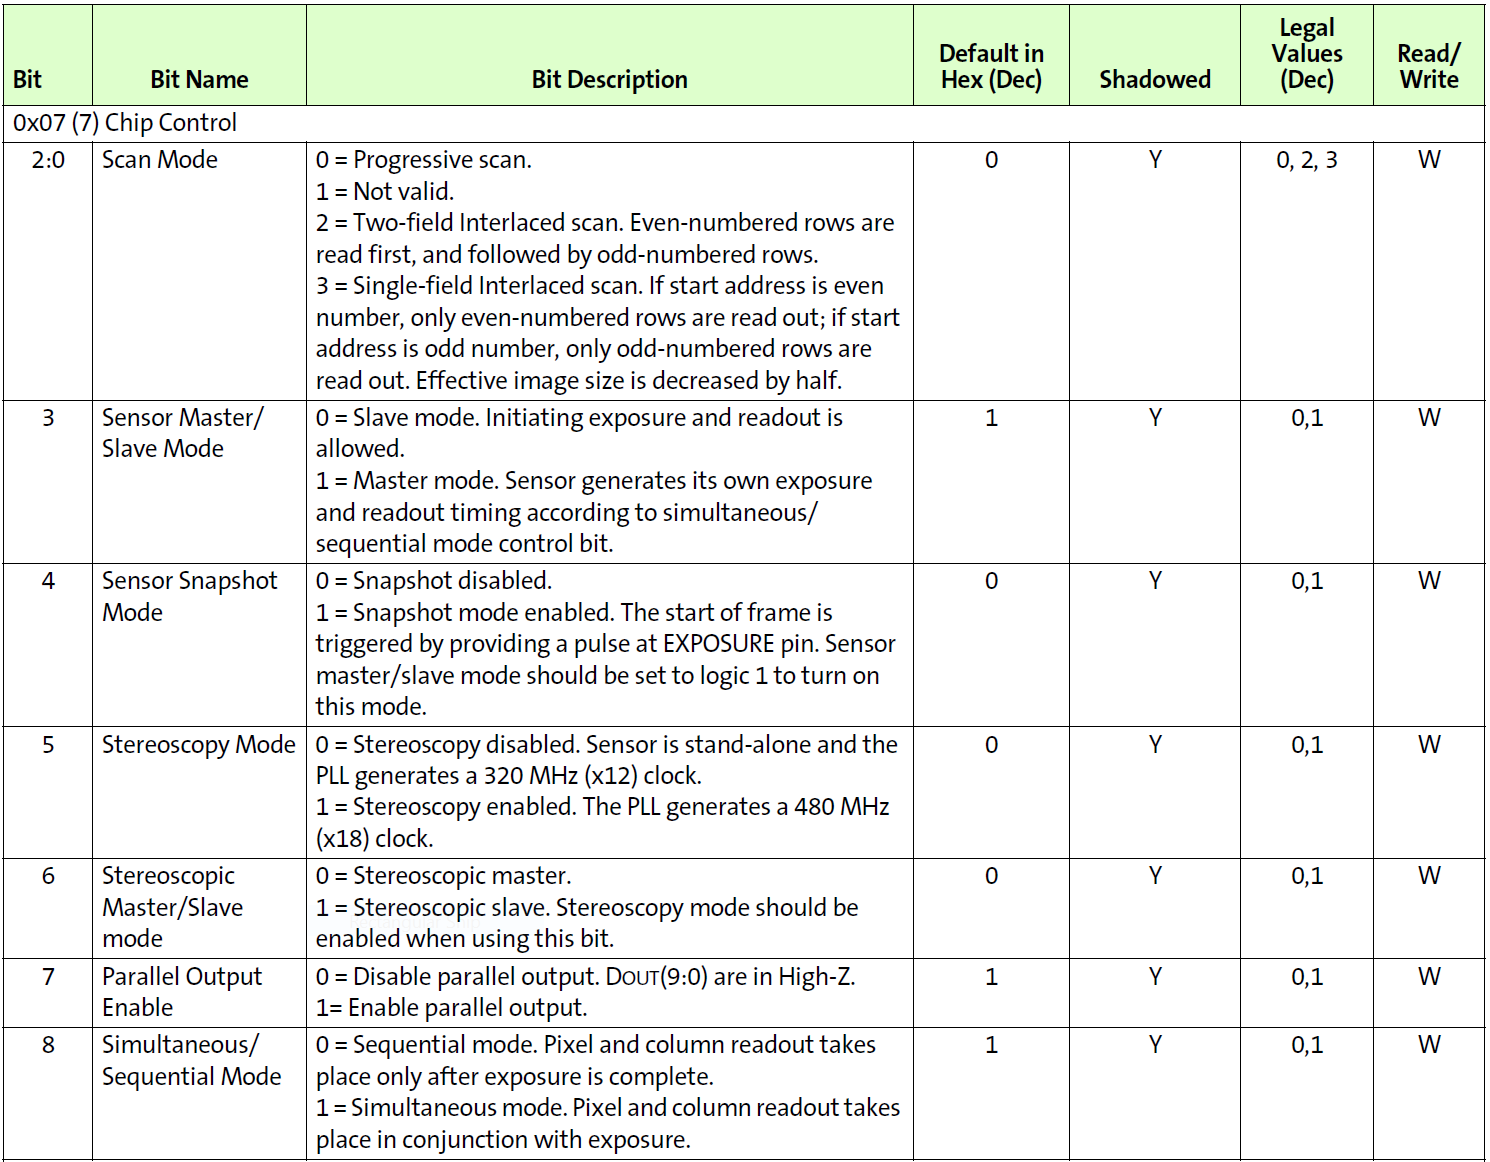
\includegraphics[width=1.0\textwidth]{CamControlReg.PNG}}
	Table obtained from MT9V032 Datasheet \cite{mt9v032}
\end{figure}
\newpage
\subsection{Stereo Camera Schematic}\label{stereoCameraSchematic}
\begin{figure}[H]
	\centerline{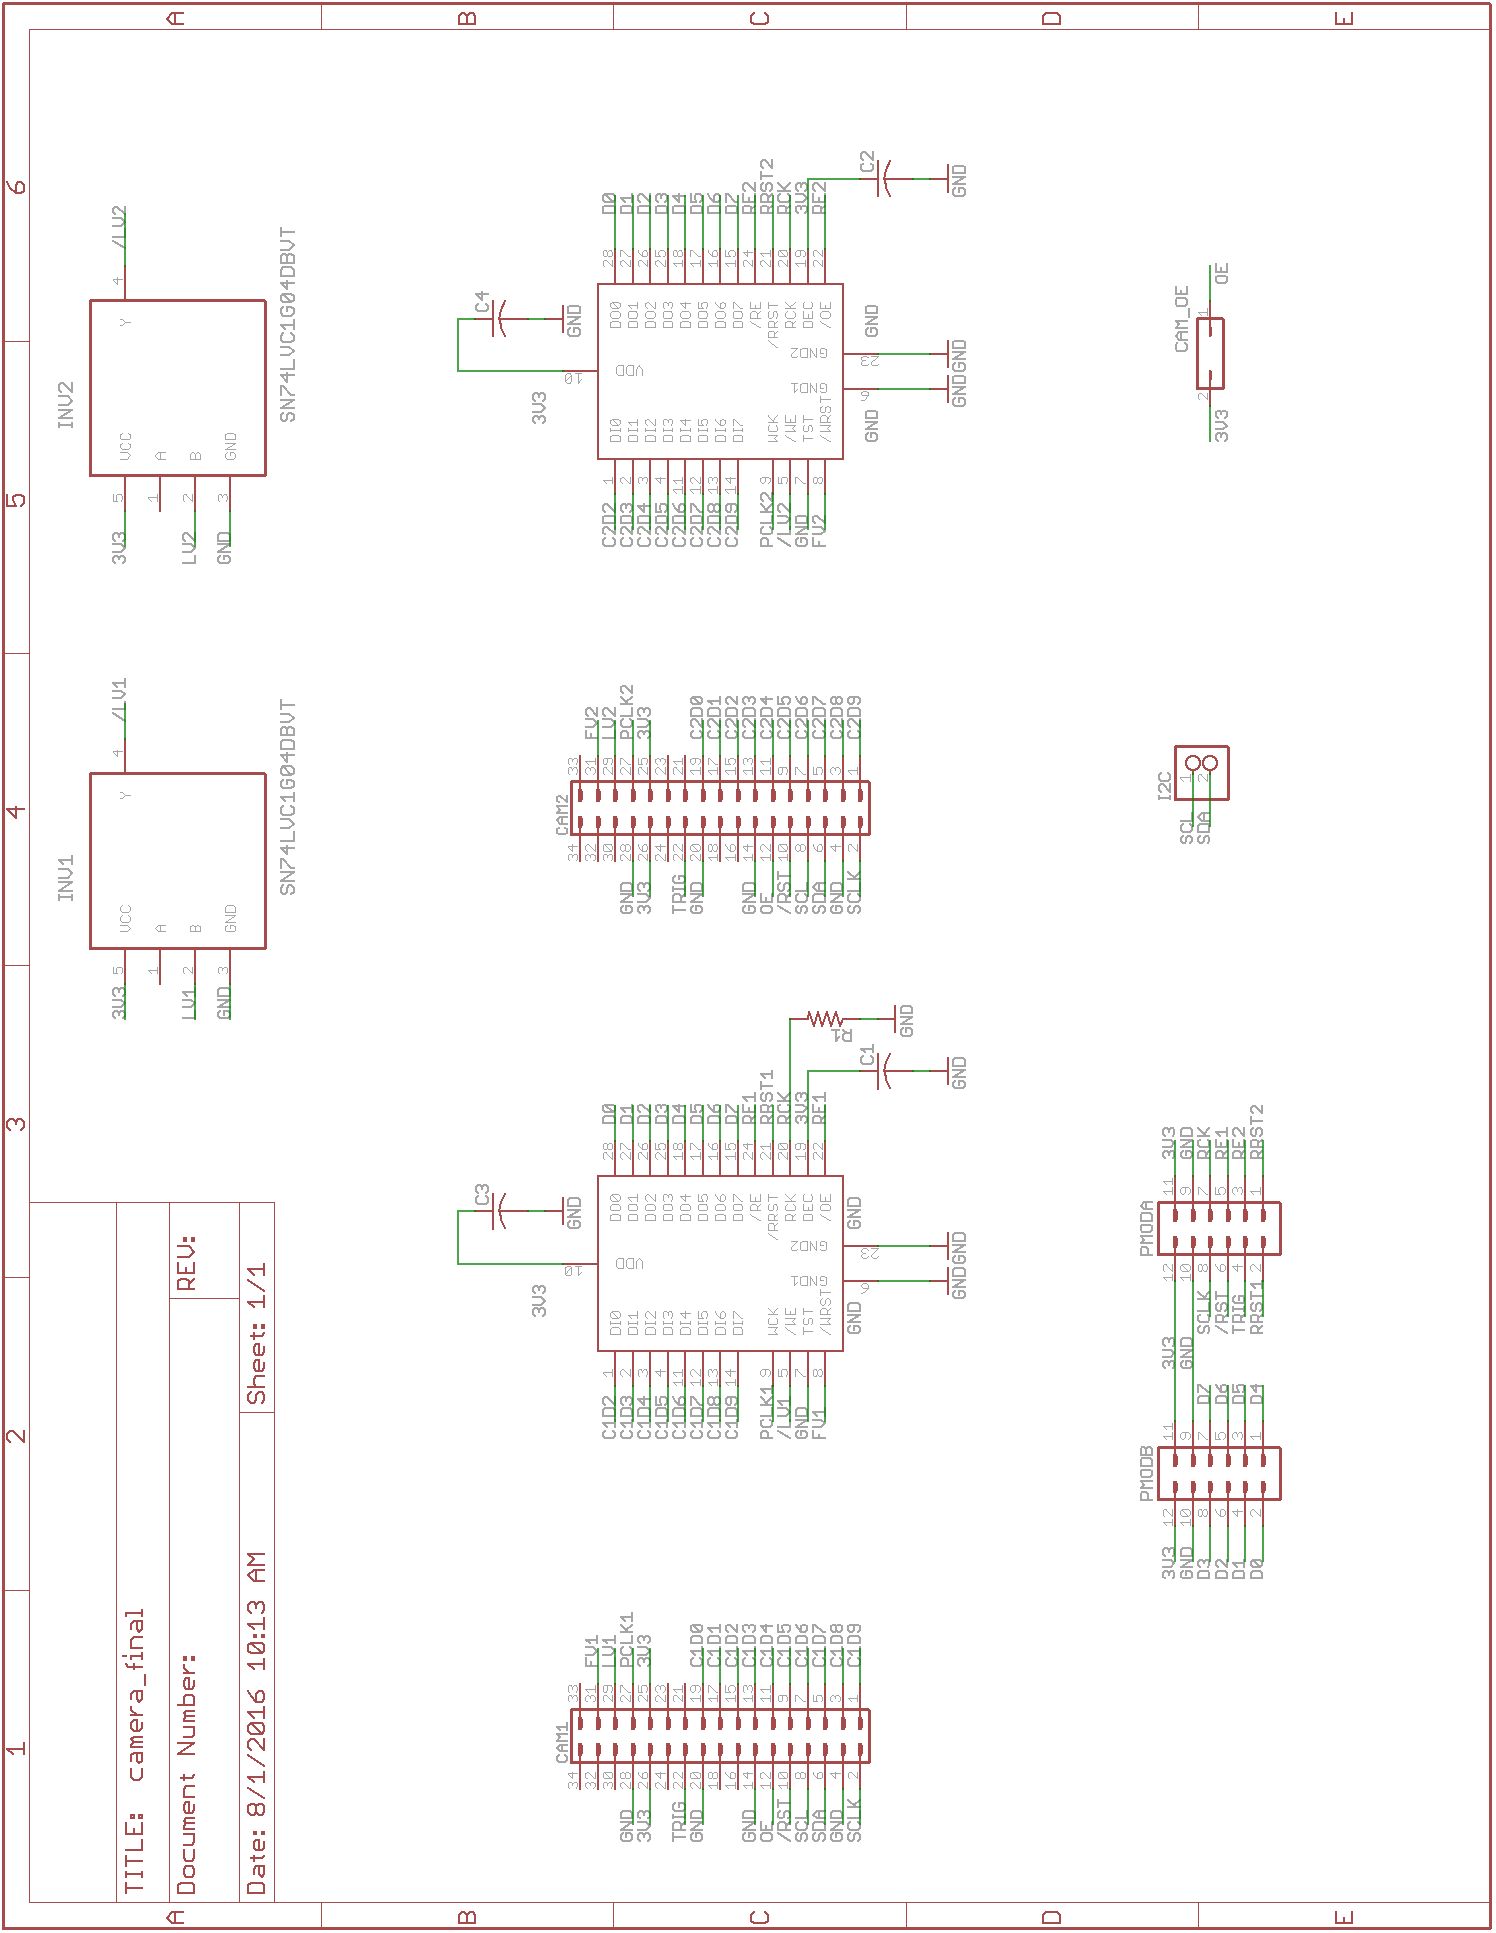
\includegraphics[width=1.0\textwidth]{stereo_schematic.png}}
\end{figure}
\newpage
\subsection{\textsc{Matlab} Code}
\subsubsection{Camera Image Parsing} \label{camTestMatlab}
\singlespacing
\lstinputlisting[style=Matlab]{appendix/matlab/ParseData.m}
\doublespacing
\newpage
\subsection{Verilog Code}
\newpage
\subsection{C Code}
\subsubsection{Camera Image Parsing} \label{camTestC}
\singlespacing
\lstinputlisting[style=C]{appendix/c/imageUART.c}
\doublespacing

\newpage
\subsection{LaTeX Coding Examples}
This section isn't intended to remain here, but can serve as an example for how to set things up later on

\subsubsection{Figures} 
\begin{figure}[H]
	\centerline{
\includegraphics[width=0.25\textwidth]{WPI_Inst_Prim_FulClr.png}}
	\caption{A Test Figure}
	\label{wpiLogo}
\end{figure}

Using the \verb!\ref! command, I'm able to reference Figure \ref{wpiLogo} by calling \verb!\ref{wpiLogo}!.

\subsubsection{Code Snippet}
Code snippets can be created by calling \verb!\begin{lstlisting}!, inserting all code, and then calling \verb!\end{lstlisting}!. Also call \verb!\singlespacing! before the code snippet and \verb!\doublespacing! after to keep things from getting too big.
\singlespacing % single space code
\begin{lstlisting}
//verilog code example
always @ (x, y, z)
  x <= y + z;
\end{lstlisting}
\doublespacing % return to double spacing after

\subsubsection{Using the bibliography}
All bibliographic references are contained in \texttt{bib.tex}. To cite a reference in the paper, use the \verb!\cite! command.
\par
As an example, I can cite \textit{Serveball} at the end of this sentence by calling \verb!\cite{serveball}!.\cite{serveball}
\par
To cite multiple references, call \verb!\cite{ref1,ref2}!.\cite{serveball,porikli}
 % example latex code for setting things up

\end{document}